\section{Preliminary studies}

This section carries out some preliminary studies using Moltres and MOOSE heat conduction module to solve the prismatic HTGR thermal-fluids.

\subsection{Verification of the thermal-fluids model}

To verify our methodology, this section solved a simplified cylindrical model whose analytical solution we know.
Section \ref{appendix:ver} presents the analytical solution of the problem.
Moltres/MOOSE obtained the numerical solution of the thermal-fluid equations from Section \ref{ch3:th}.

Figure \ref{fig:th-ver-mesh} displays the model geometry, which differentiates five subregions: fuel compact, helium gap, moderator, film, and coolant.
Table \ref{tab:th-ver-char} summarizes the geometry dimensions and the input parameters.
The model reference design was the GT-MHR.
The calculated moderator radius is the fuel/coolant pitch minus the fuel compact and coolant channel radii, which is the minimum distance between the fuel and coolant channels in the unit cell.
We obtained the calculated coolant radius by preserves the coolant channel volume.
The model assumed a sinusoidal power profile in the $z$-direction.

\begin{figure}[htbp!]
	\centering
	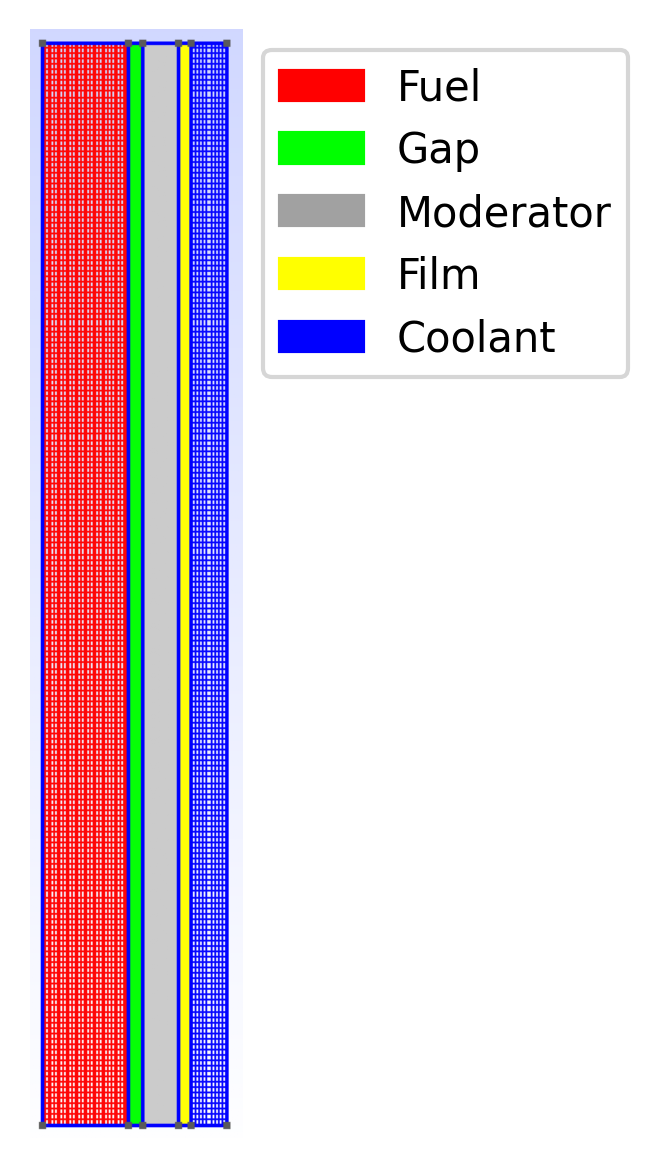
\includegraphics[width=0.25\linewidth]{figures-thermal/2D-preliminar-mesh2}
	\hfill
	\caption{Scaled-down version of the model geometry.}
	\label{fig:th-ver-mesh}
\end{figure}

\begin{table}[htbp!]
\centering
      \caption{Problem characteristics.}
      \label{tab:th-ver-char}
    % \begin{tabular}{@{}l c S[table-format=2.2] c c}
    \begin{tabular}{@{}l c c c c}
    \toprule
    \multicolumn{1}{c}{Parameter} & \multicolumn{1}{c}{Symbol} & \multicolumn{1}{c@{}}{Value} & \multicolumn{1}{c@{}}{Units} & \multicolumn{1}{c}{Reference} \\
    \midrule
  Fuel compact radius   & R$_f$     & 0.6225  & cm       & \cite{in_three-dimensional_2006} \\
  Fuel channel radius   & R$_g$     & 0.6350  & cm       & \cite{in_three-dimensional_2006} \\
  Coolant channel radius   & - 		& 0.7950  & cm       & \cite{in_three-dimensional_2006} \\
  Fuel/coolant pitch    & -			& 1.8850  & cm       & \cite{in_three-dimensional_2006} \\
  Fuel column height	& L 		& 793 	  & cm 		 & \cite{in_three-dimensional_2006} \\
  Coolant mass flow rate & $\dot{m}$ & 0.0176 & kg/s 	 & \cite{in_three-dimensional_2006} \\
  Average power density & q$_{ave}$ & 35      & W/cm$^3$ & \cite{in_three-dimensional_2006} \\
  Coolant inlet temperature 	& $T_{in}$ & 400  & $^{\circ}C$ & \cite{in_three-dimensional_2006} \\
  Helium inlet pressure & P 		& 70      & bar 	 & \cite{in_three-dimensional_2006} \\
  Helium density		& $\rho_c$  & 4.940 $\times 10^{-6}$ & kg/cm$^3$ & \cite{nist_thermophysical_2020} \\
  Helium heat capacity  & c$_{p,c}$	& 5188 & J/kg/K  & \cite{nist_thermophysical_2020} \\
  Fuel compact thermal conductivity & k$_f$ & 0.07    & W/cm/K & \cite{tak_numerical_2008} \\
  Gap thermal conductivity & k$_g$ & 3 $\times 10^{-3}$ & W/cm/K & \cite{tak_numerical_2008} \\
  Moderator thermal conductivity & k$_m$ & 0.30 & W/cm/K 	& \cite{tak_numerical_2008} \\
    \midrule
  \multicolumn{1}{c}{Calculated parameters} &  &  &  & \\  
    \midrule
  Calculated moderator radius 	& R$_m$ & 1.080  	& cm     & - \\
  Coolant film radius   		& R$_i$ & 1.090  	& cm     & - \\
  Calculated coolant radius 	& R$_c$ & 1.349  	& cm     & - \\
  Coolant average velocity  	& v$_c$ & 1794.33 	& cm/s   & - \\
  Film thermal conductivity  	& k$_i$ & 1.722 $\times 10^{-3}$ & W/cm/K & - \\
  \bottomrule
  \end{tabular}
\end{table}

Figure \ref{fig:th-ver-results} shows the axial and radial temperature profiles.
Both analytical and numerical solutions exhibit good agreement.
The outlet coolant temperature is 770.2 $^{\circ}$C whereas the average outlet coolant temperature of the VHTR is 950 $^{\circ}$C.
Note that this is a simplified model only for verification purposes, and it considers only one fuel channel while in the GT-MHR unit cell two fuel channels deposit their heat into one coolant channel.

\begin{figure}[htbp!]
	\centering
    \subfloat[Fuel centerline and bulk coolant axial temperatures.]{
        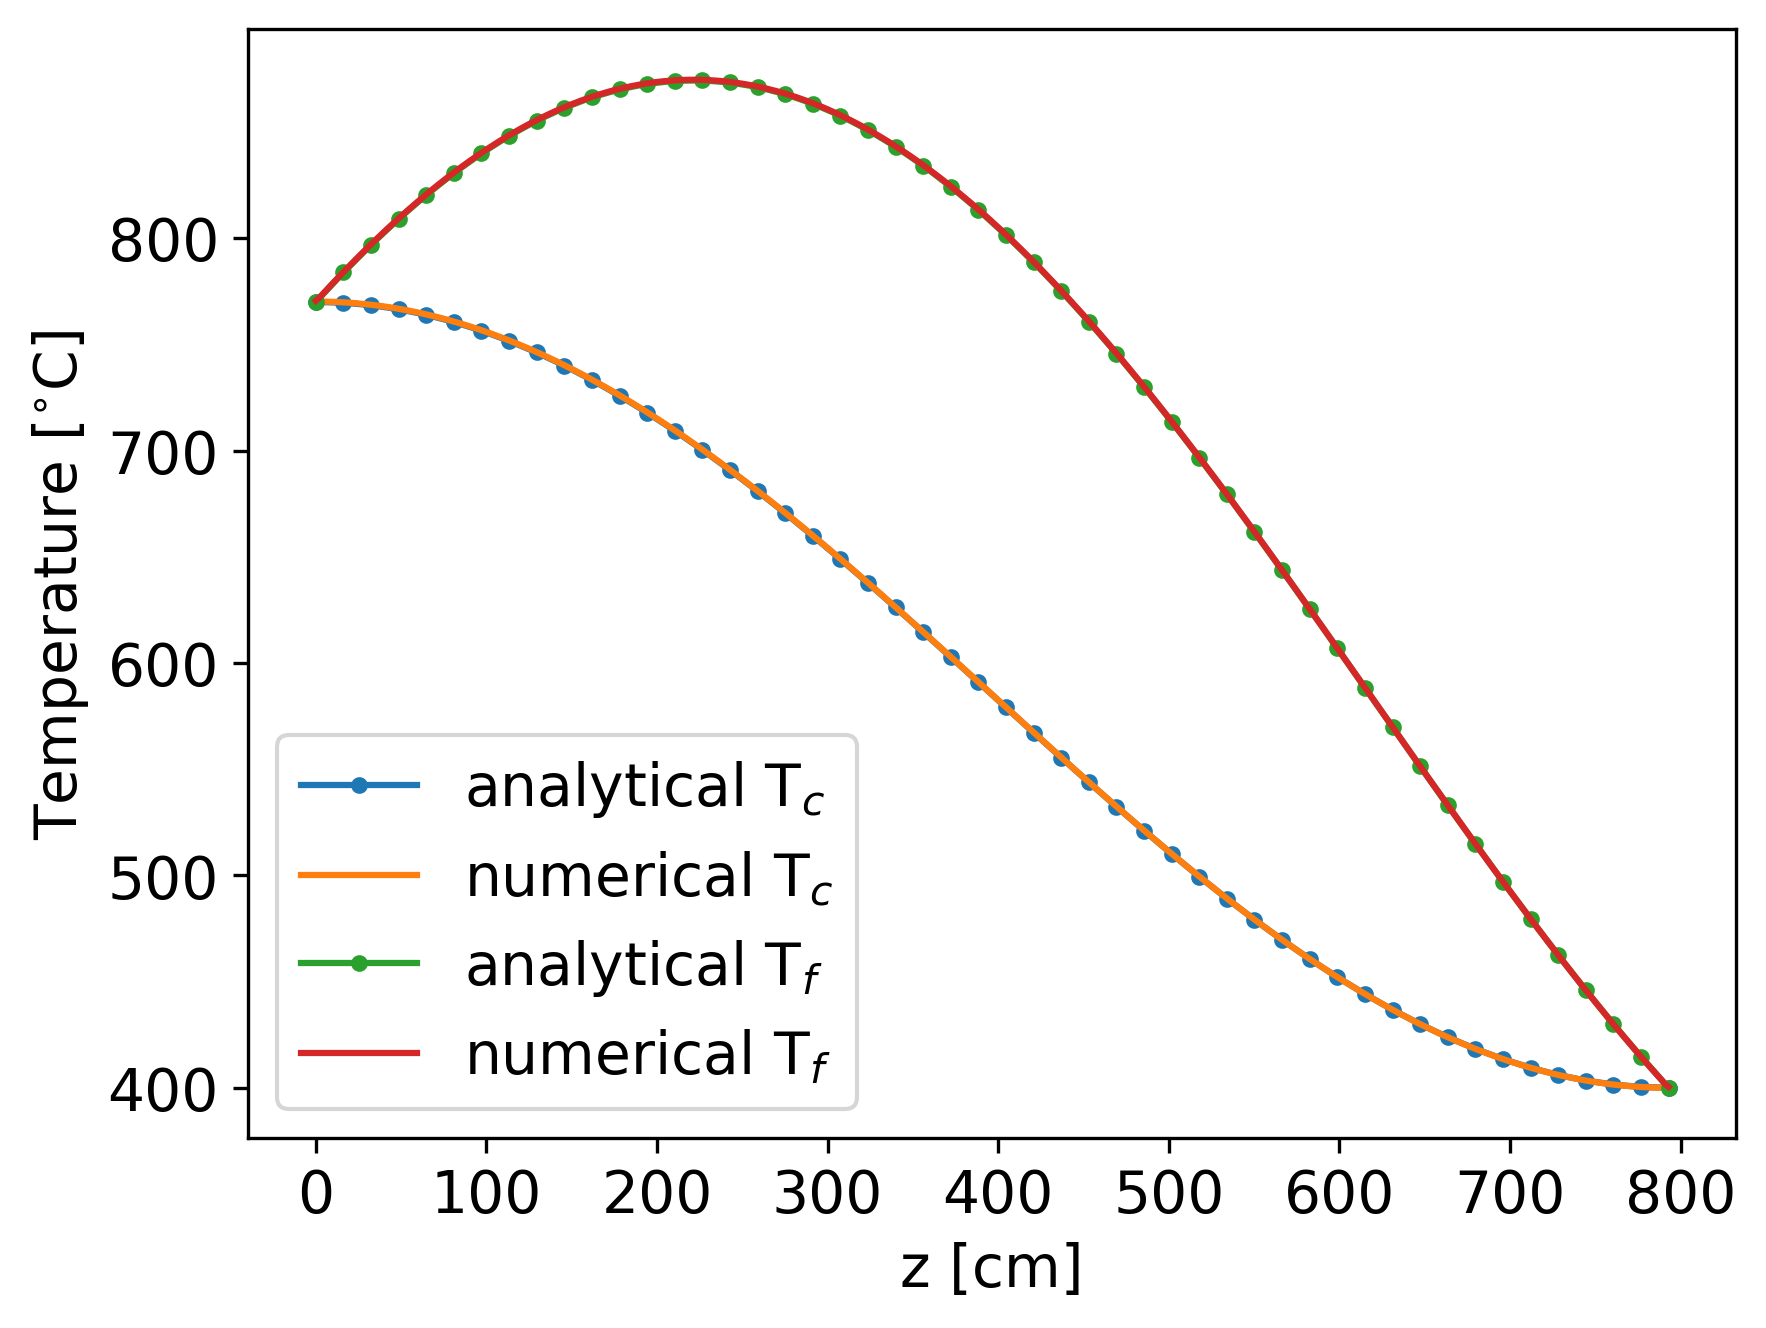
\includegraphics[width=0.45\textwidth]{figures-thermal/2D-preliminar-axial}
    }
    \subfloat[Radial temperature at z=L/2=396.5 cm.]{
        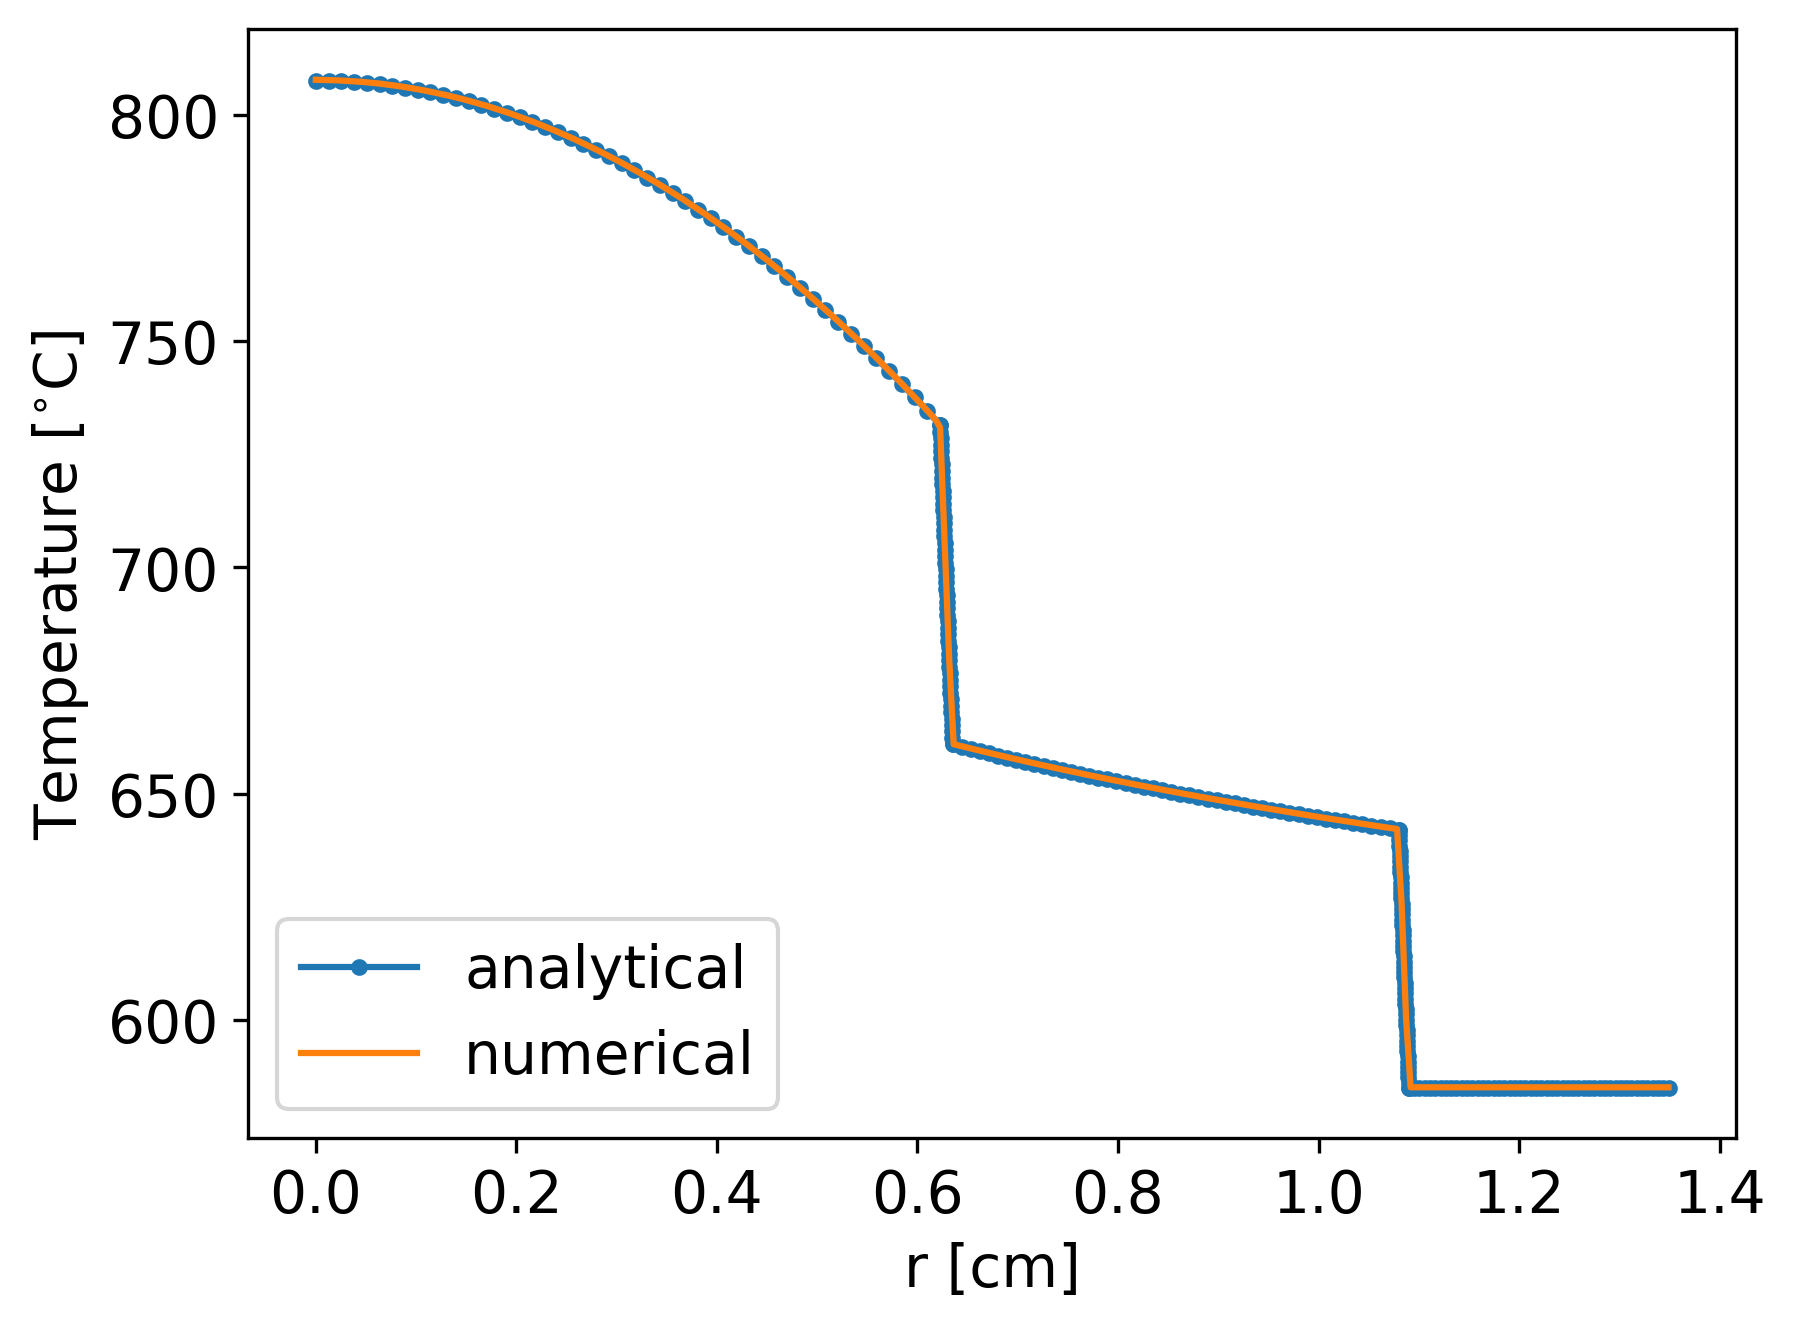
\includegraphics[width=0.45\textwidth]{figures-thermal/2D-preliminar-radial2}
    }
	\hfill
    \caption{Temperature profiles.}
	\label{fig:th-ver-results}
\end{figure}

\section{Unit cell problem}

This section solved the unit cell problem in the hot spot of an HTGR.
We intended to reproduce In et al. 2006 \cite{in_three-dimensional_2006} in an effort to validate the unit-cell model.
We chose this article as it solves a three-dimensional unit-cell model and gives one of the most complete descriptions in the open literature.
Table \ref{tab:th-val-unit-char} presents the problem characteristics.
The material properties specification of the solids is missing in the article, and we replaced them with parameters from Tak et al. 2008 \cite{tak_numerical_2008}.
Figure \ref{fig:th-val-unit-model} displays a $XY$-plane of the model geometry and the material properties that depend on the temperature.
Additionally, In et al. used a chopped cosine as the power profile.
To simplify the analysis, we used the average value of the power profile.

\begin{table}[htbp!]
\centering
      \caption{Problem characteristics.}
      \label{tab:th-val-unit-char}
    % \begin{tabular}{@{}l c S[table-format=2.2] c c}
    \begin{tabular}{@{}l c c c c}
    \toprule
    \multicolumn{1}{c}{Parameter} & \multicolumn{1}{c}{Symbol} & \multicolumn{1}{c@{}}{Value} & \multicolumn{1}{c@{}}{Units} & \multicolumn{1}{c}{Reference} \\
    \midrule
  Fuel compact radius       & R$_f$ & 0.6225    & cm   & \cite{in_three-dimensional_2006} \\
  Fuel channel radius       & R$_g$ & 0.6350    & cm   & \cite{in_three-dimensional_2006} \\
  Coolant channel radius    & R$_c$ & 0.7950    & cm   & \cite{in_three-dimensional_2006} \\
  Fuel/coolant pitch        & p     & 1.8850    & cm   & \cite{in_three-dimensional_2006} \\
  Fuel column height        & L     & 793       & cm   & \cite{in_three-dimensional_2006} \\
  % input parameter characteristics
  Coolant channel mass flow rate & $\dot{m}$ & 0.0176 & kg/s & \cite{in_three-dimensional_2006} \\
  Average power density     & q$_{ave}$ & 35    & W/cm$^3$   & \cite{in_three-dimensional_2006} \\
  Inlet coolant temperature & T$_{in}$  & 400   & $^{\circ}$C  & \cite{in_three-dimensional_2006} \\
  Helium inlet pressure & P & 70 & bar & \cite{in_three-dimensional_2006} \\
  Helium density        & $\rho$  & 4.94 $\times 10^{-6}$ & kg/cm$^3$ & \cite{nist_thermophysical_2020} \\
  Helium heat capacity  & c$_p$ & 5188 & J/kg/K & \cite{nist_thermophysical_2020} \\
    \midrule
  \multicolumn{1}{c}{Calculated parameters} &  &  &  & \\  
    \midrule
  Coolant film radius       & R$_i$ & 0.8050    & cm     & -  \\
  Coolant average velocity  & v$_c$ & 1794.33   & cm/s   & -  \\
  Film thermal conductivity & k$_i$ & 1.731 $\times 10^{-3}$ & W/cm/K & -  \\
  \bottomrule
  \end{tabular}
\end{table}

\begin{figure}[htbp!]
	\centering
    \subfloat[Model geometry.]{
        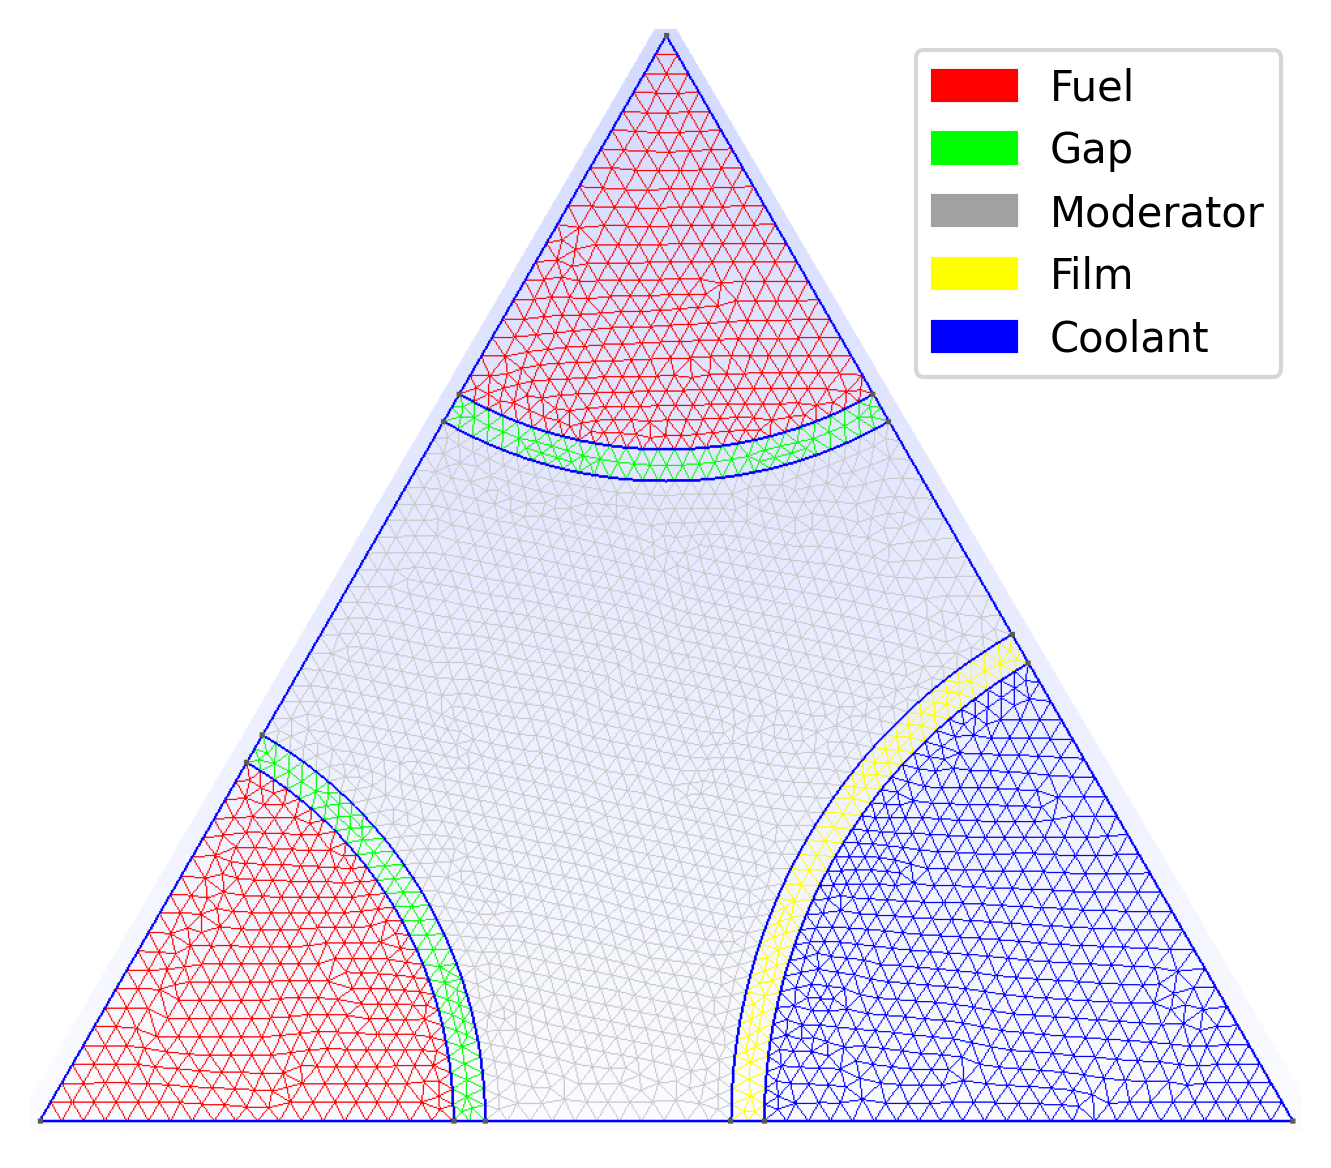
\includegraphics[width=0.40\textwidth]{figures-thermal/val-unit-mesh}
    }
    \subfloat[Material properties.]{
        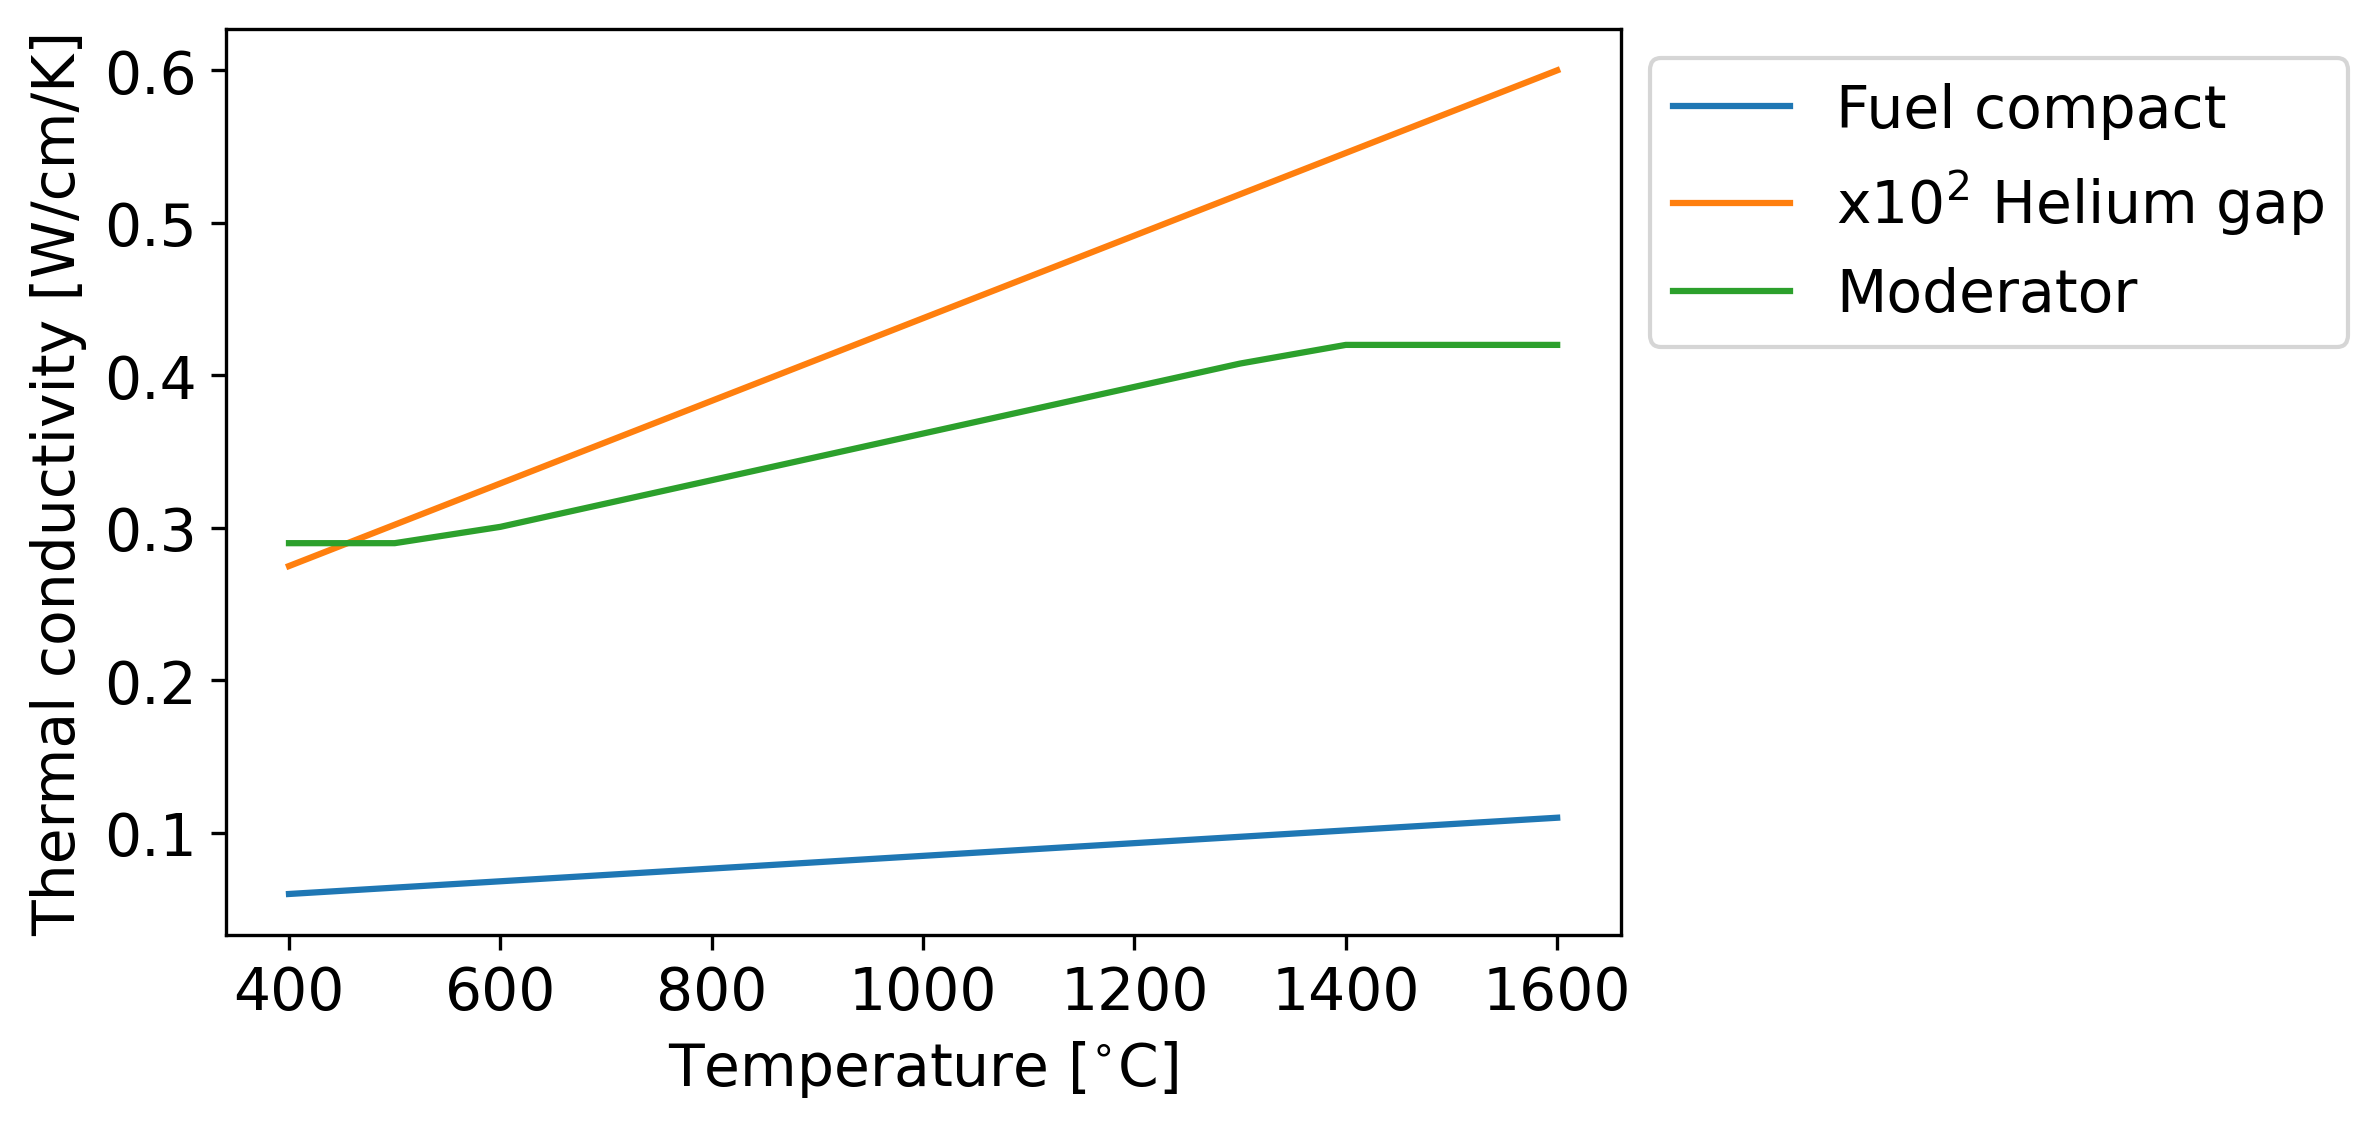
\includegraphics[width=0.50\textwidth]{figures-thermal/val-unit-matprop}
    }
	\hfill
  \caption{Moltres/MOOSE input parameters.}
	\label{fig:th-val-unit-model}
\end{figure}

Figure \ref{fig:th-val-unit-temps} shows the temperature profiles.
The axial temperatures increase from the top to the bottom of the reactor.
The moderator and coolant temperatures are parallel as the model assumes a film thermal conductivity independent of the temperature.
The fuel and moderator temperature difference decreases.
As the thermal conductivities of the different materials increase with temperature, the thermal resistance between the moderator and the fuel decreases.
Table \ref{tab:th-val-unit-results} summarizes the results.
Moltres/MOOSE coolant temperature is smaller by 4$^{\circ}$C.
The moderator temperature is larger by 9$^{\circ}$C.
The fuel temperature is larger by 22$^{\circ}$C.
The cause of this is the power profile simplification.
For a sinusoidal power profile the fuel-to-coolant temperature difference is small in the outlet, as we have seen in the previous section.
The opposite scenario is the uniform power profile, where the fuel-to-coolant temperature difference is larger.
In et al. used a chopped cosine power profile which we can think of it as the case in between a uniform and a sinusoidal power profile.
Overall, our model results showed good agreement with In et al. results.

\begin{figure}[htbp!]
  \centering
    \subfloat[Maximum fuel, moderator, and bulk coolant axial temperatures.]{
        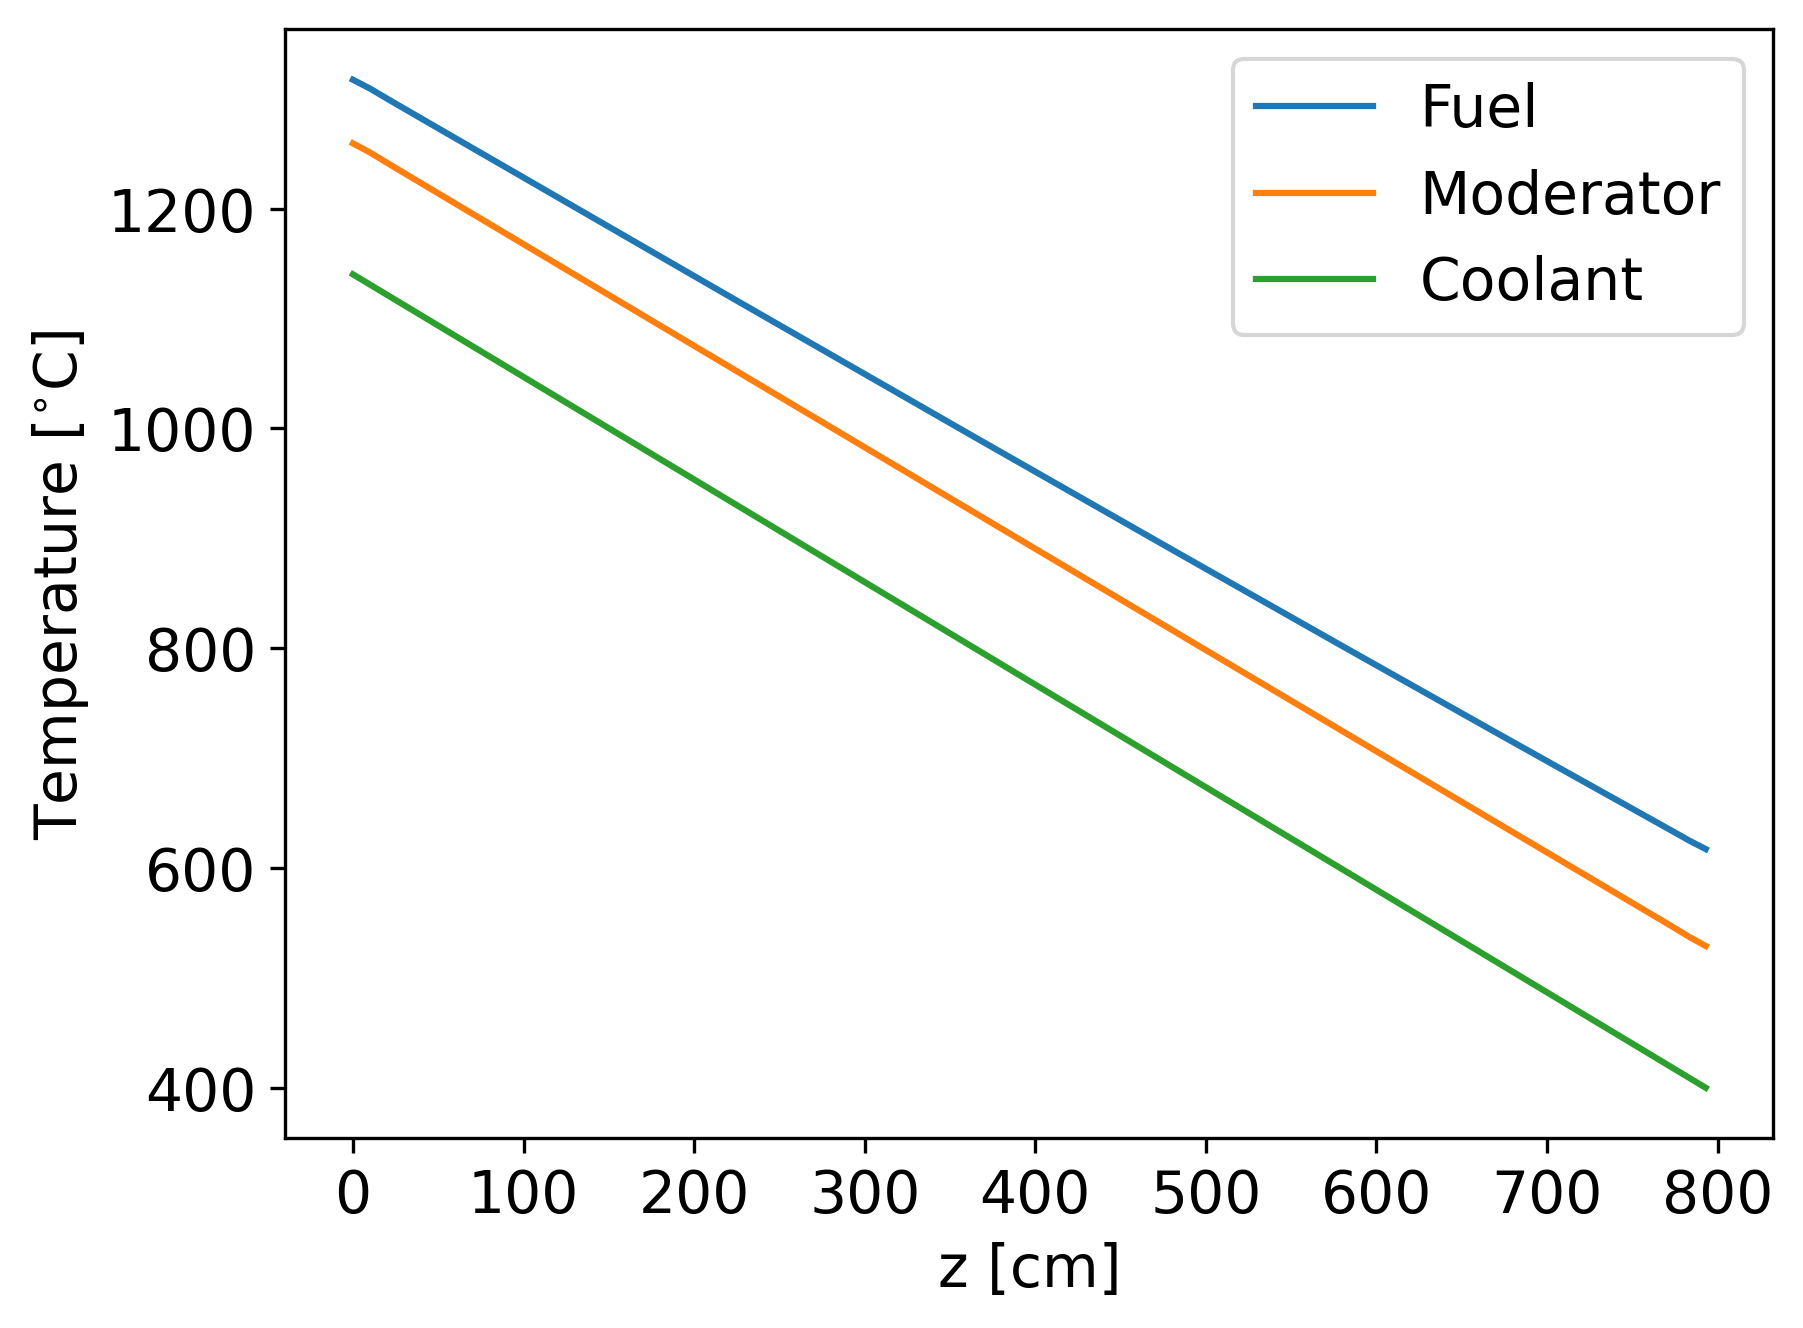
\includegraphics[width=0.45\textwidth]{figures-thermal/in-2006-5-axial}
    }
    \subfloat[Outlet plane temperature z=793 cm.]{
        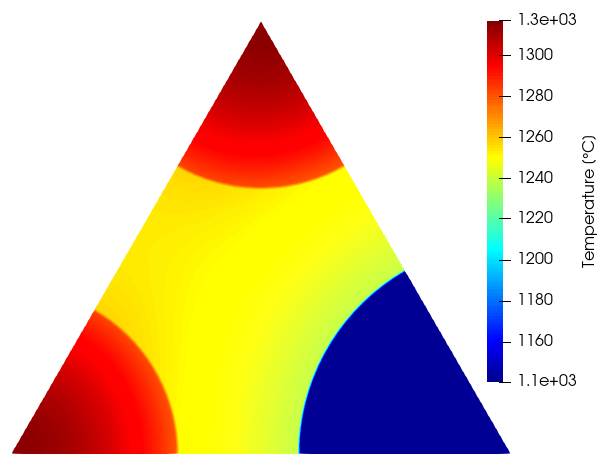
\includegraphics[width=0.45\textwidth]{figures-thermal/val-unit-outlet-plane}
    }
  \hfill
  \caption{Temperature profiles.}
  \label{fig:th-val-unit-temps}
\end{figure}

\begin{table}[htbp!]
\centering
    \caption{Maximum temperatures.}
    \label{tab:th-val-unit-results}
    \begin{tabular}{@{}l c c}
    \toprule
  Parameter   & In et al. 2006 \cite{in_three-dimensional_2006} & Moltres/MOOSE \\
    \midrule
  Maximum coolant temperature [$^{\circ}$C]   & 1144 & 1140 \\
  Maximum moderator temperature [$^{\circ}$C] & 1250 & 1259 \\
  Maximum fuel temperature [$^{\circ}$C]      & 1295 & 1317 \\
    \bottomrule
  \end{tabular}
\end{table}

\section{Fuel column}

This section solved an HTGR fuel column.
It aimed to reproduce some of the analyses in Sato et al. 2010 \cite{sato_computational_2010} in an effort to validate the fuel column model.
We chose this article as it gives a thorough description of the problem making it easier to reproduce.
First, we analyzed a case with no bypass-gap.
Second, we studied a case with a 3mm-gap.

The study used the GT-MHR as the reference reactor for the calculations.
Figure \ref{fig:th-val-assem-model-a} exhibits the model geometry.
The model included only a one-twelfth portion of the column due to symmetry.
The GT-MHR shares the geometry specifications with the MHTGR.
Table \ref{tab:element-characteristics} specifies the fuel element geometry.

Equation \ref{eq:matcoeff} describes the solid material properties \cite{johnson_cfd_2009}.
Table \ref{tab:th-val-assem-mat} displays the fuel compact and moderator thermal conductivities coefficients.
Table \ref{tab:th-val-assem-char} lists several input parameters, including the helium properties.
Figure \ref{fig:th-val-assem-model-b} shows the temperature dependent material properties.

\begin{align}
  \phi(T) = A_1 + A_2 T + A_3 T^2 + A_4 T^3 + A_5 T^4  \label{eq:matcoeff}
\end{align}

The model assigns a number to each coolant channel and the bypass-gap, see Figure \ref{fig:th-val-assem-model-a}.
In this exercise, we use the mass flow distribution from Sato et al.
Table \ref{tab:th-val-assem-massflow} shows the mass flow rate in each channel.

\begin{table}[htbp!]
\centering
      \caption{Problem characteristics.}
      \label{tab:th-val-assem-char}
    % \begin{tabular}{@{}l c S[table-format=2.2] c c}
    \begin{tabular}{@{}l c c c c}
    \toprule
    \multicolumn{1}{c}{Parameter} & \multicolumn{1}{c}{Symbol} & \multicolumn{1}{c@{}}{Value} & \multicolumn{1}{c@{}}{Units} & \multicolumn{1}{c}{Reference} \\
    \midrule
  Inlet coolant temperature & T$_{in}$  & 490   & $^{\circ}$C   & \cite{sato_computational_2010} \\
  Helium inlet pressure     & P         & 70    & bar           & \cite{sato_computational_2010} \\
  Helium density            & $\rho$    & 4.37 $\times 10^{-6}$ & kg/cm$^3$ & \cite{nist_thermophysical_2020} \\
  Helium heat capacity      & c$_p$     & 5188  & J/kg/K        & \cite{nist_thermophysical_2020} \\
  Average power density     & q$_{ave}$ & 27.88 & W/cm$^3$      & \cite{sato_computational_2010} \\
    \midrule
  \multicolumn{1}{c}{Calculated parameters} &  &  &  & \\  
    \midrule
  Coolant film radius       & R$_i$ & 0.804    & cm     & -  \\
  Film thermal conductivity & k$_i$ & 2.09 $\times 10^{-3}$ & W/cm/K & -  \\
  \bottomrule
  \end{tabular}
\end{table}

\begin{table}[htbp!]
\centering
  \caption{Thermal conductivity coefficients.}
  \label{tab:th-val-assem-mat} 
  \begin{tabular}{c|ccc|c}
\toprule
                          & \multicolumn{3}{c|}{Moderator}         & Fuel compact \\ \hline
Temperature range {[}K{]} & 255.6-816 & 816-1644.4 & 1644.4-1922.2 & 255.6-2200   \\
\midrule
A1                        & 28.6      & 1.24E+2    & 41.5          & 3.94         \\
A2                        & -         & -3.32E-1   & -             & 3.59E-3      \\
A3                        & -         & 4.09E-4    & -             & -1.98E-9     \\
A4                        & -         & -2.11E-7   & -             & 3.19E-12     \\
A5                        & -         & 4.02E-11   & -             & -9.77E-16    \\
\bottomrule
  \end{tabular}
\end{table}

% maybe see this to center the figures
% https://tex.stackexchange.com/questions/121824/horizontal-centering-with-subfloat

\begin{figure}[htbp!]
  \centering
    \subfloat[Model geometry. \label{fig:th-val-assem-model-a}]{
        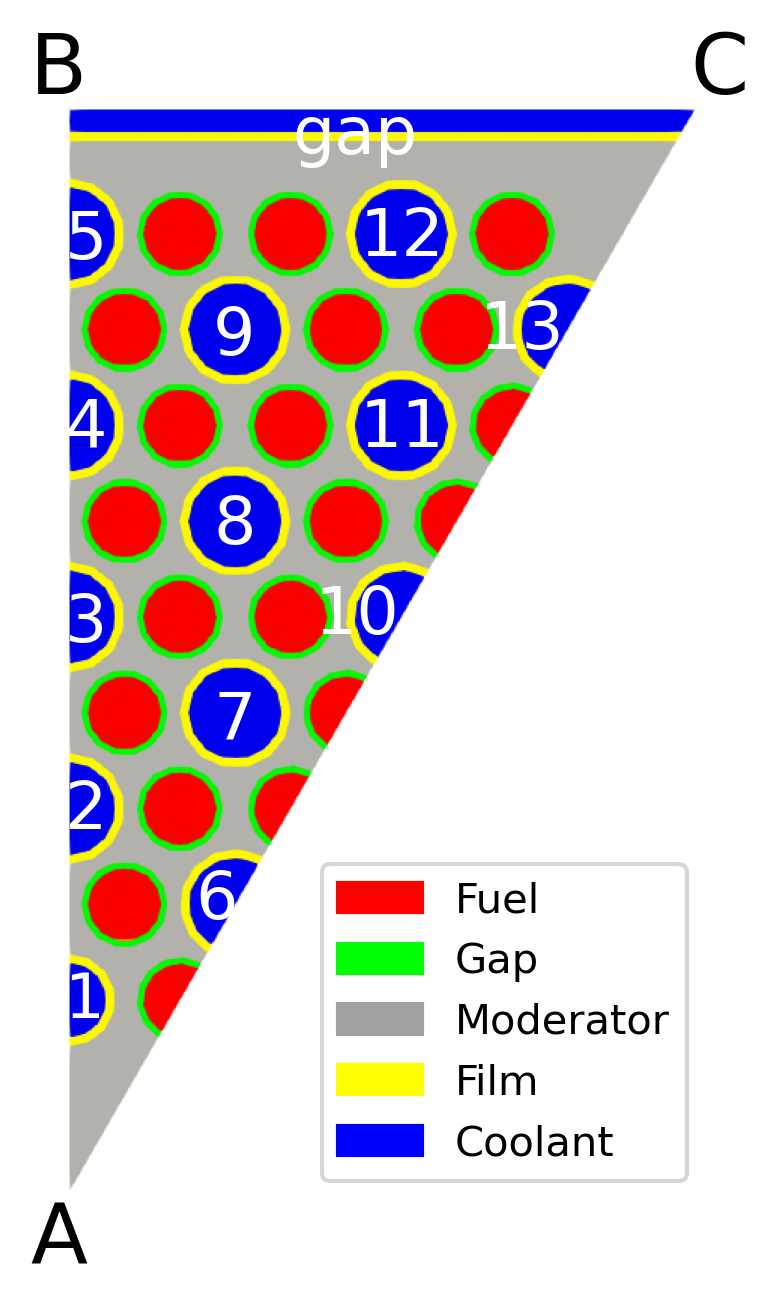
\includegraphics[width=0.25\textwidth]{figures-thermal/val-assem-mesh}
    }
    \subfloat[Material properties. \label{fig:th-val-assem-model-b}]{
        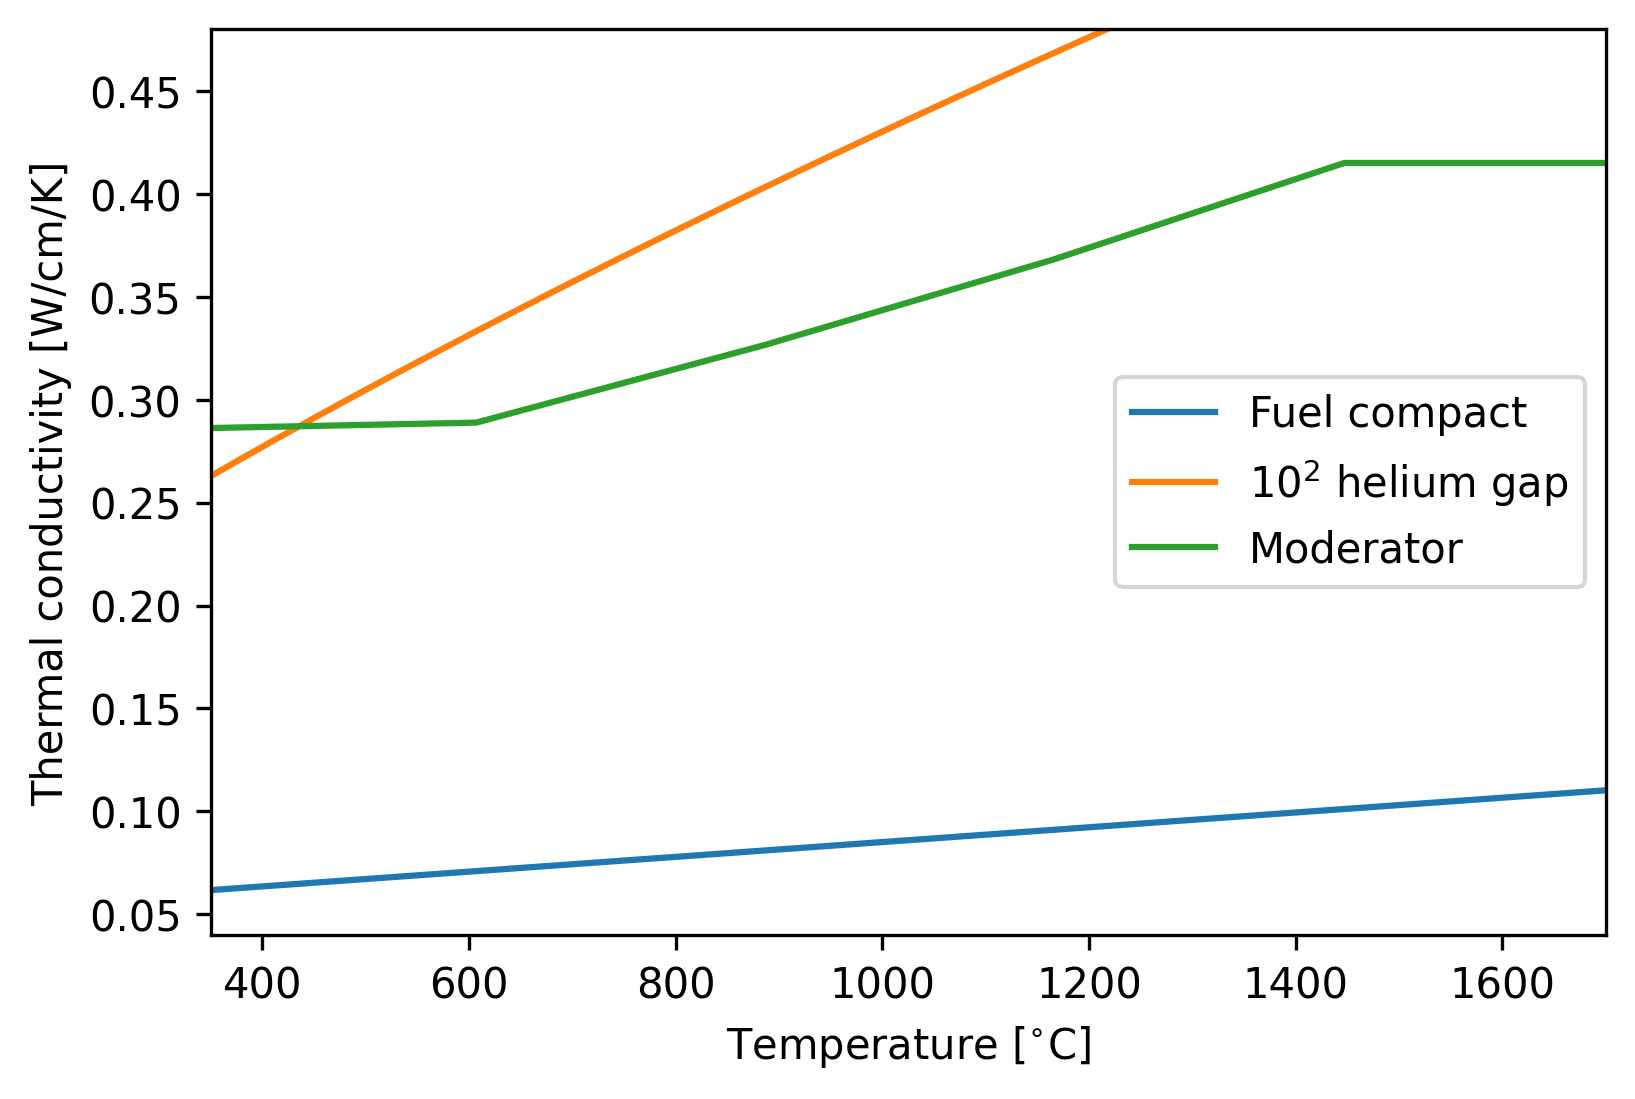
\includegraphics[width=0.45\textwidth]{figures-thermal/val-assem-matprop}
    }
  \hfill
  \label{fig:th-val-assem-model}
\end{figure}

% \begin{table}[htbp!]
% \centering
%   \caption{Mass flow rate [g/s]. Values form \cite{sato_computational_2010}.}
%   \label{tab:th-val-assem-massflow}
%   \begin{tabular}{l|llllllllllllll}
% \toprule
% Channel & 1 & 2 & 3 & 4 & 5 & 6 & 7 & 8 & 9 & 10 & 11 & 12 & 13 & Gap \\
% \midrule
% No gap  & 6.18 & 11.34 & 11.37 & 11.38 & 11.43 & 11.33 & 22.70 & 22.73 & 22.73 & 11.38 & 22.77 & 22.91 & 11.44 & -     \\
% 3mm gap & 5.88 & 10.80 & 10.85 & 10.91 & 11.08 & 10.80 & 21.58 & 21.67 & 21.83 & 10.88 & 21.81 & 22.20 & 11.10 & 16.56 \\
% \bottomrule
% \end{tabular}
% \end{table}

\begin{table}[htbp!]
\centering
  \caption{Mass flow rate [g/s]. Values form \cite{sato_computational_2010}.}
  \label{tab:th-val-assem-massflow}
  \begin{tabular}{l|lllllll}
\toprule
Channel & 1 & 2 & 3 & 4 & 5 & 6 & 7 \\
\midrule
No gap  & 6.18 & 11.34 & 11.37 & 11.38 & 11.43 & 11.33 & 22.70 \\
3mm gap & 5.88 & 10.80 & 10.85 & 10.91 & 11.08 & 10.80 & 21.58 \\
\midrule
Channel & 8 & 9 & 10 & 11 & 12 & 13 & Gap \\
\midrule
No gap  & 22.73 & 22.73 & 11.38 & 22.77 & 22.91 & 11.44 & -     \\
3mm gap & 21.67 & 21.83 & 10.88 & 21.81 & 22.20 & 11.10 & 16.56 \\
\bottomrule
\end{tabular}
\end{table}

Table \ref{tab:th-val-assem-results} compares Moltres/MOOSE results to the Sato's results.
In the no gap case, Moltres/MOOSE's maximum bulk coolant temperature is 2 $^{\circ}$C lower and the maximum fuel temperature is 4$^{\circ}$C higher.
In the 3mm-gap case, Moltres/MOOSE's maximum bulk coolant temperature is 2 $^{\circ}$C lower and the maximum fuel temperature is 1$^{\circ}$C lower.
The results showed good agreement.

Figure \ref{fig:th-val-assem-temps} displays the outlet temperature along lines A-B and A-C from Figure \ref{fig:th-val-assem-model-a}.
The temperature is higher closer to the column center.
The bypass-flow causes the temperature in the center to rise while reducing the peripheral temperature.
The presence of the gap produces a larger temperatures gradient in the assembly.

\begin{table}[htbp!]
  \centering
  \caption{Maximum temperatures.}
  \label{tab:th-val-assem-results}
\begin{tabular}{l|c|c|c|c}
\toprule
        & \multicolumn{2}{c|}{No gap} & \multicolumn{2}{c}{3mm gap} \\ \cline{2-5}
        & Sato et al. & Moltres/MOOSE & Sato et al. & Moltres/MOOSE \\ \midrule
Bulk coolant & 985     & 983               & 1007     & 1005             \\  
Fuel    & 1090    & 1094              & 1115     & 1114             \\
\bottomrule
\end{tabular}
\end{table}

\begin{figure}[htbp!]
  \centering
  % \hspace*{\fill}
    \subfloat[Line A-B.]{
        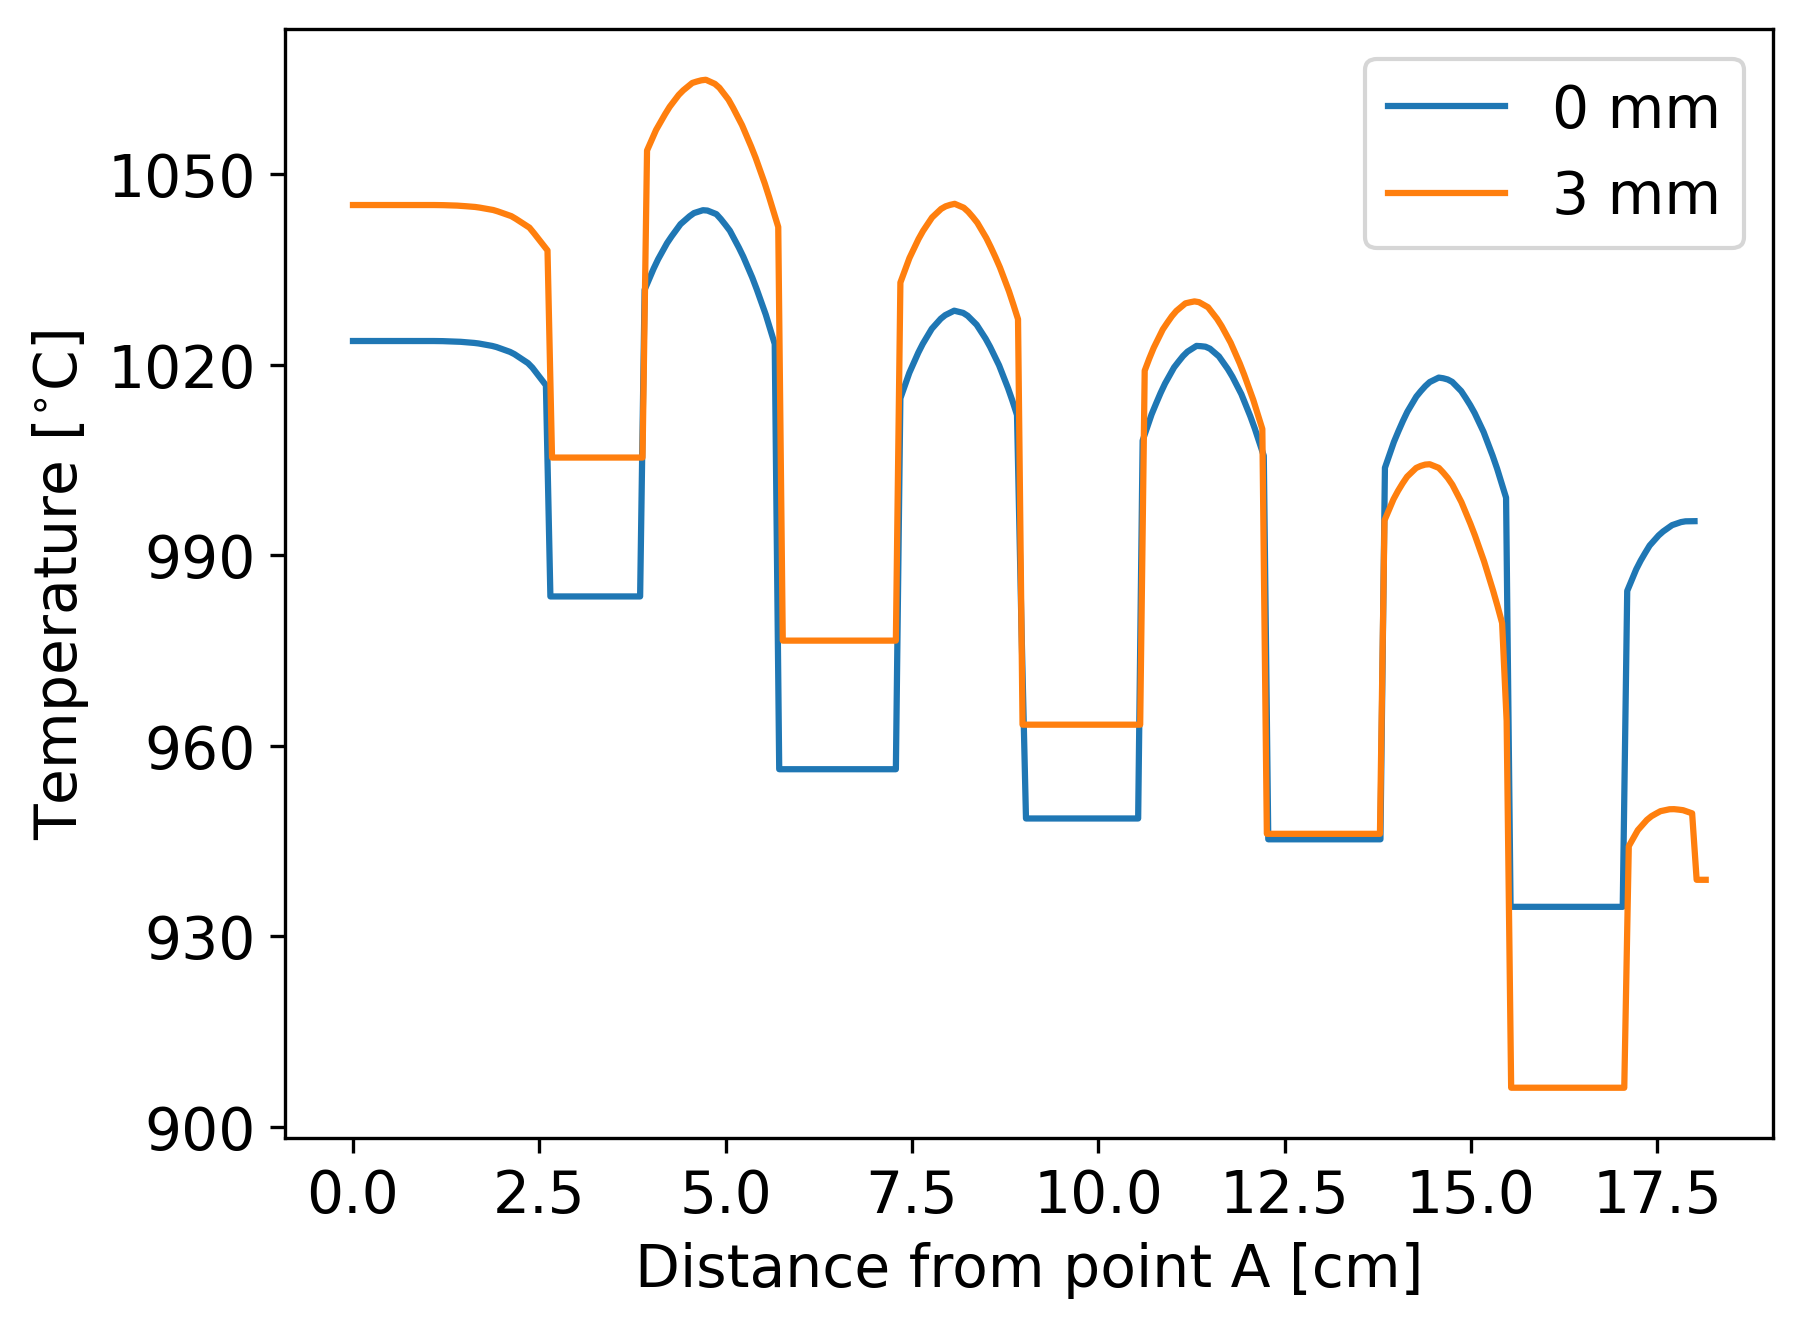
\includegraphics[width=0.45\textwidth]{figures-thermal/val-assem-line-AB}
    }
    \subfloat[Line A-C.]{
        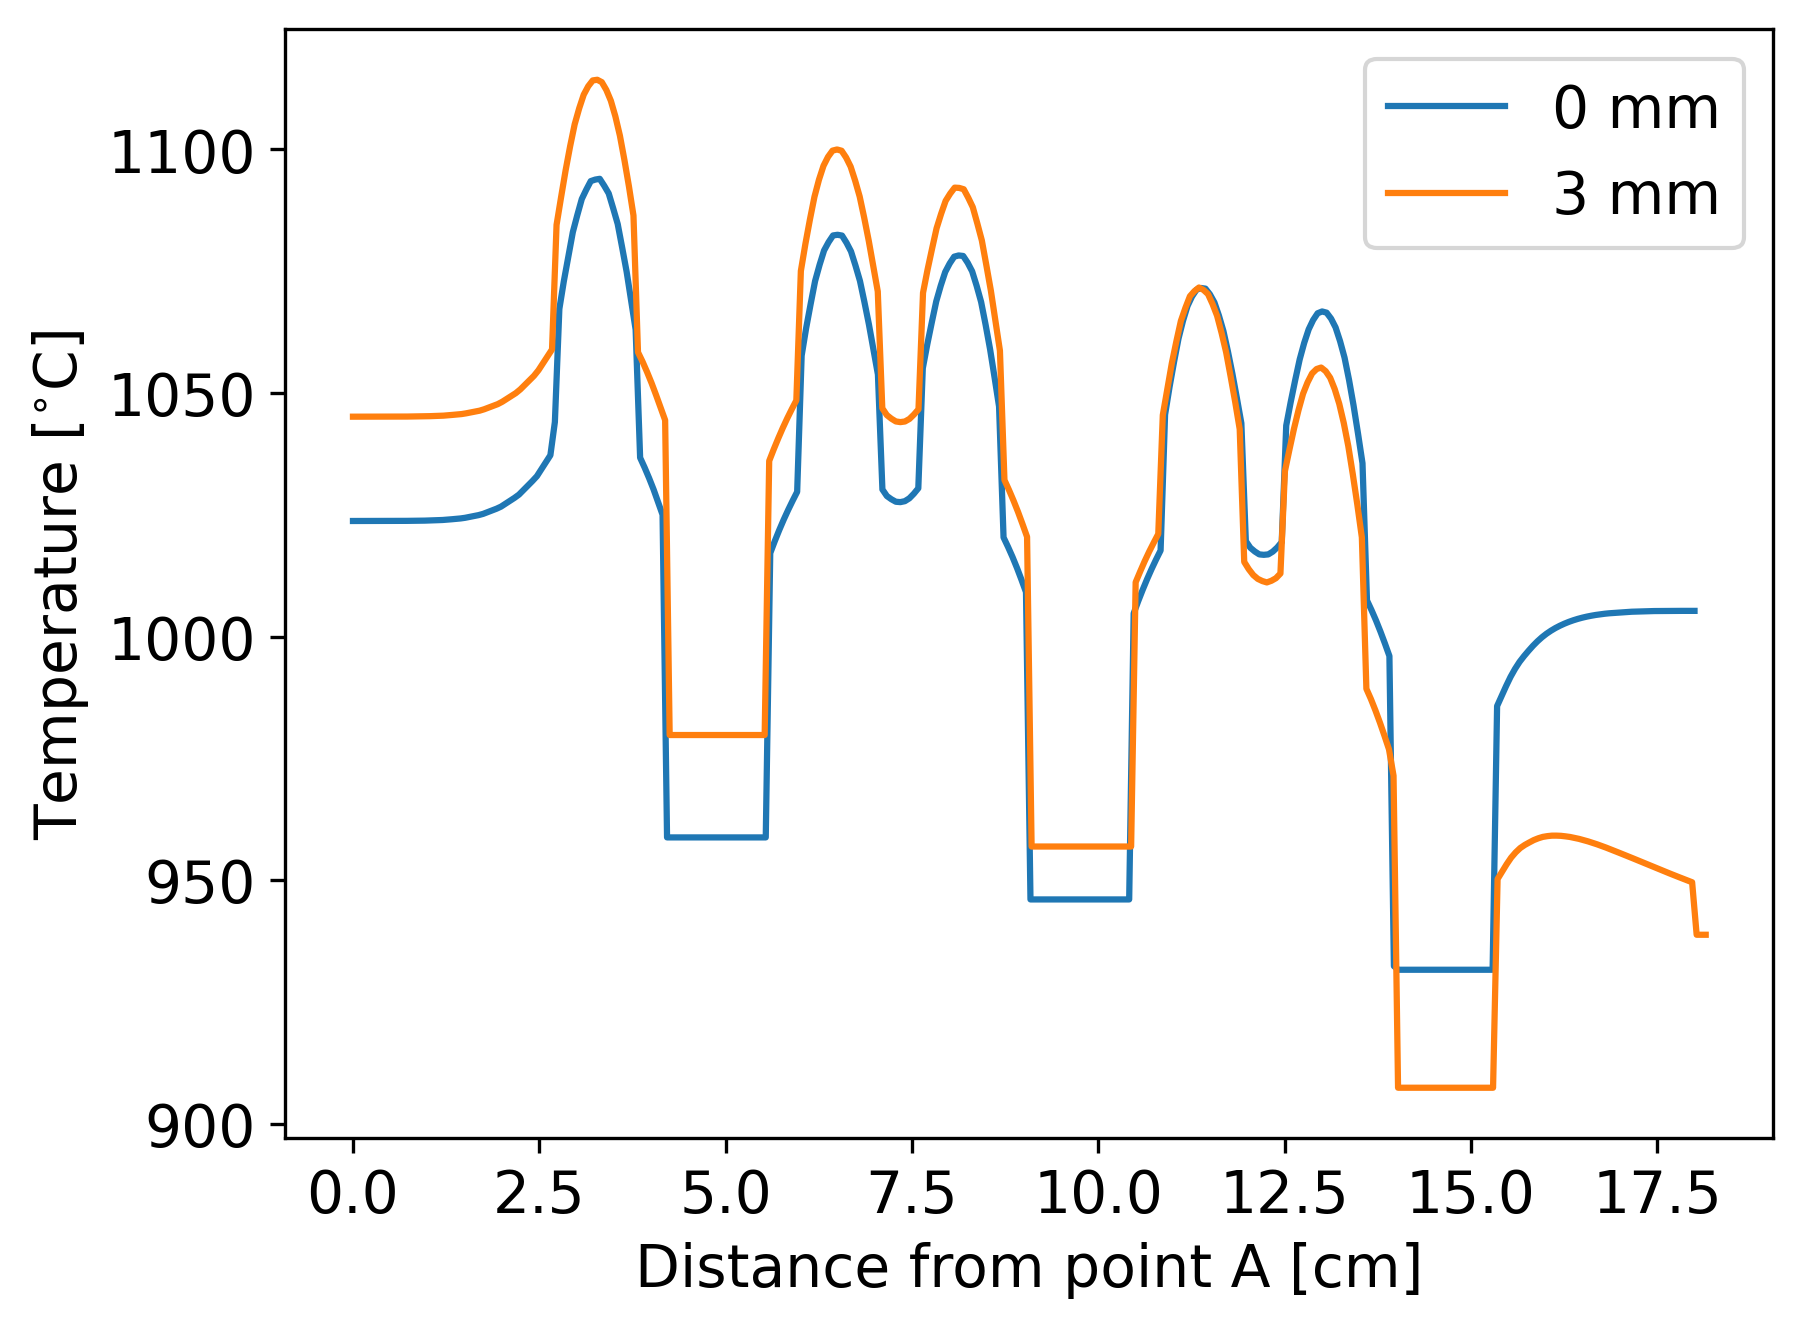
\includegraphics[width=0.45\textwidth]{figures-thermal/val-assem-line-AC}
    }
  \hfill
  \caption{Outlet plane temperature along the line A-B and line A-C.}
  \label{fig:th-val-assem-temps}
\end{figure}

% \begin{figure}[htbp!]
%   \centering
%     \subfloat[No gap.]{
%         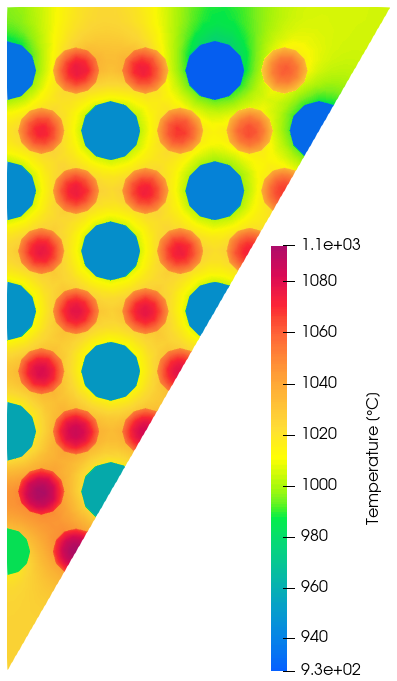
\includegraphics[width=0.45\textwidth]{figures-thermal/val-assem-input}
%     }
%     \subfloat[3mm gap.]{
%         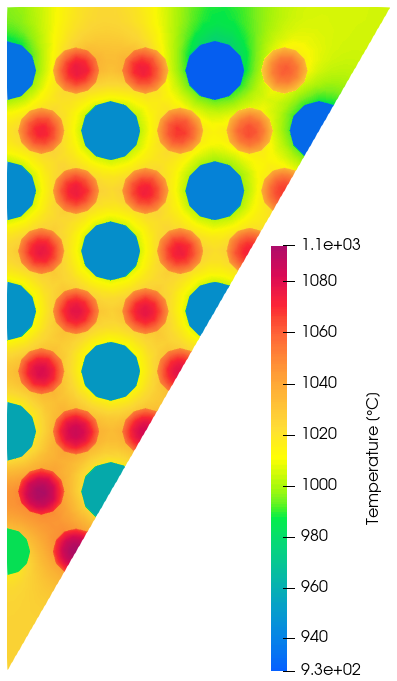
\includegraphics[width=0.45\textwidth]{figures-thermal/val-assem-input}
%     }
%   \hfill
%   \caption{Outlet plane temperature profile.}
%   \label{fig:th-val-assem-temps}
% \end{figure}

\subsection{Flow distribution analysis}

As mentioned in Section \ref{sec:litrev-thermalf} several authors calculate the flow distribution using various methods.
This section compares the effects of different methods on the results.
To carry out such comparison, the chosen metrics are the maximum coolant and fuel temperatures and the mass flow distribution.
The model assigns a number to each coolant channel and the bypass-gap, see Figure \ref{fig:th-val-assem-model-a}.
Note that channel 1 is a small coolant channel while channels 2 to 13 are large coolant channels.

We analyzed the following cases:
\begin{itemize}
    \item Case 1: uses the mass flow distribution from Sato et al.
    \item Case 2: uses a flat velocity profile (every channel and gap has the same velocity).
    \item Case 3: uses the incompressible flow model with a temperature independent helium viscosity.
    \item Case 4: uses the incompressible flow model with a temperature dependent helium viscosity.
    \item Case 5: uses the low-Mach number model with a temperature dependent helium viscosity.
\end{itemize}

To calculate the different cases flow distribution, we used the following equations.
Equation \ref{eq:case2mdot} calculated the flow distribution in case 1.
Equation \ref{eq:case3mdot} \cite{melese_thermal_1984} calculated the pressure drop in cases 3 and 4.
Case 4 differs from case 3 as the friction factor $f$ depends on the average channel temperature.
Equation \ref{eq:case5mdot} \cite{melese_thermal_1984} calculated the pressure drop in case 5.
For cases 3 to 5, the pressure drop is proportional to the channel mass flow, equation \ref{eq:itersolver1}.
Equations \ref{eq:case3mdot} and \ref{eq:case5mdot} calculated $B_i$.
Equations \ref{eq:itersolver2} and \ref{eq:itersolver3} solved the mass flow distribution iteratively.
As cases 4 and 5 mass flow distributions depend on the temperature, the calculations required a few iterations to obtain the final mass flow distribution.
The convergence criteria was 1$^{\circ}$C for the maximum coolant and fuel temperatures.

\begin{align}
  \dot{m}_i &= \frac{A_i}{\sum_j A_j} \label{eq:case2mdot} \\
  \Delta P &= \frac{1}{\rho} \left( \frac{\dot{m}_i}{A_i} \right)^2 f \frac{2 L}{D_h} \label{eq:case3mdot} \\
  \Delta P &= \frac{\dot{m}_i^2}{2 \rho A_i^2} \left[ \frac{4 f L (T_i+T_o)}{2 D T_i} + \frac{T_o-T_i}{T_i} \right]  \label{eq:case5mdot} \\
  \Delta P &= B_i \dot{m}_i^2 \label{eq:itersolver1} \\
  \Delta P &= \left( \frac{\dot{m}_T}{\sum_i \frac{1}{\sqrt{B_i}}} \right)^2 \label{eq:itersolver2} \\
  \dot{m}_i &= \sqrt{\Delta P / B_i} \label{eq:itersolver3}
  \intertext{where}
  \dot{m}_i &= \mbox{channel $i$ mass flow rate} \notag \\
  A_i &= \mbox{channel $i$ cross-sectional area} \notag \\
  \Delta P &= \mbox{pressure drop} \notag \\
  T_i &= \mbox{channel inlet coolant temperature} \notag \\
  T_o &= \mbox{channel outlet coolant temperature} \notag \\
  \dot{m}_T &= \mbox{total mass flow rate} \notag \\
\end{align}

Table \ref{tab:th-assem-flow-massflow} displays the mass flow rates.
Case 4 and case 5 converged after two and three iterations, respectively.
Case 2 yields the largest small coolant channel mass flow, and the smallest large coolant channel mass flow.
Case 3 and 4 barely differ.
Not taking into account the temperature dependency of the viscosity yields a simpler method and the accuracy loss is negligible.
Case 5 arrives to the closest values to the reference solution.

Table \ref{tab:th-assem-flow-results} summarizes the maximum temperatures.
For the maximum coolant temperature. case 2 yields the largest difference which is smaller than less than 10$^{\circ}$C.
Case 5 yields the best result.
For the maximum fuel temperature, case 2 and 5 yield the best results.
Again, case 3 and 4 barely differ.

The low-Mach number model yielded the closest results to the reference solution.
However, such method required an iterative solver.
From a computational point of view, case 2 model is the simplest method as it does not require an iterative solver.
Additionally, case 2 model yields the simplest Moltres/MOOSE input file.
For these reasons, the rest of the thesis uses case 2 model for the fluid flow distribution.

\begin{table}[htbp!]
  \centering
  \caption{Mass flow rates [g/s].}
  \label{tab:th-assem-flow-massflow}
  \begin{tabular}{l|llllllllllllll}
\toprule
Channel & 1 & 2 & 3 & 4 & 5 & 6 & 7 \\
\midrule
Case 1  & 5.88 & 10.80 & 10.85 & 10.91 & 11.08 & 10.80 & 21.58 \\
Case 2  & 6.66 & 10.41 & 10.41 & 10.41 & 10.41 & 10.41 & 20.82 \\
Case 3  & 5.98 & 10.91 & 10.91 & 10.91 & 10.91 & 10.91 & 21.82 \\
Case 4  & 5.97 & 10.90 & 10.90 & 10.91 & 10.92 & 10.90 & 21.80 \\
Case 5  & 5.83 & 10.75 & 10.81 & 10.90 & 11.09 & 10.73 & 21.58 \\
\midrule
Channel & 8 & 9 & 10 & 11 & 12 & 13 & Half-gap \\
\midrule
Case 1  & 21.67 & 21.83 & 10.88 & 21.81 & 22.20 & 11.10 & 8.28 \\
Case 2  & 20.82 & 20.82 & 10.41 & 20.82 & 20.82 & 10.41 & 8.20 \\
Case 3  & 21.82 & 21.82 & 10.91 & 21.82 & 21.82 & 10.91 & 8.55 \\
Case 4  & 21.81 & 21.83 & 10.91 & 21.82 & 21.85 & 10.92 & 8.55 \\
Case 5  & 21.71 & 21.92 & 10.84 & 21.87 & 22.26 & 11.08 & 8.63 \\
\bottomrule
\end{tabular}
\end{table}

\begin{table}[htbp!]
  \centering
  \caption{Maximum temperatures.}
  \label{tab:th-assem-flow-results}
\begin{tabular}{l|lllll}
\toprule
                            & Case 1 & Case 2 & Case 3 & Case 4 & Case 5 \\
\midrule
Maximum coolant temperature & 1005   &  994   &  999 & 1000 & 1007 \\
Maximum fuel temperature    & 1114   & 1116   & 1109 & 1110 & 1116 \\
\bottomrule
\end{tabular}
\end{table}

% Conclusion: not sure about this
This simplified algorithms allow for solving the mass flow rate distribution in the core for steady-state cases, and for transient cases as an approximation.
However, in coupled analyses, the flow distribution depends on the temperature and will change along time.
This creates the necessity for developing tools integrated into Moltres.
Currently, MOOSE has a module for modeling the incompressible Navier-Stokes equations.
Integrating that module into the solver could improve the accuracy.
This task will be part of the future work.

\section{Mesh convergence analysis}
% I might not include this in the final document

In the remainder of this Chapter, we intend to solve the full-core problem.
This section aims to identify some possible problems introduced by a large mesh size requirement.
This section conducts a mesh convergence analysis of the full-column problem.
Figure \ref{fig:th-full-assem-mesh} displays the model geometry.
Table \ref{tab:th-full-assem-results} presents the results.
The convergence criteria was 1$^{\circ}$C for the maximum coolant and fuel temperatures.
The coolant temperature converges for the fifth mesh.
The fuel temperature did not reach convergence.
Further refinement of the mesh was not possible as the simulation memory requirements were to high.

This analysis reveals a problem.
The high level of detail in our geometry requires a large number of elements in the mesh.
Moving forward, the problem dimensions will increase and will do so too the number of elements in the mesh.
Potentially, this method will not be able to solve the three-dimensional full scale problem due to a high memory requirement.
For this reason, the next section intends to solve the full scale problem using a two-dimensional cylindrical model.

\begin{figure}[htbp!]
  \centering
  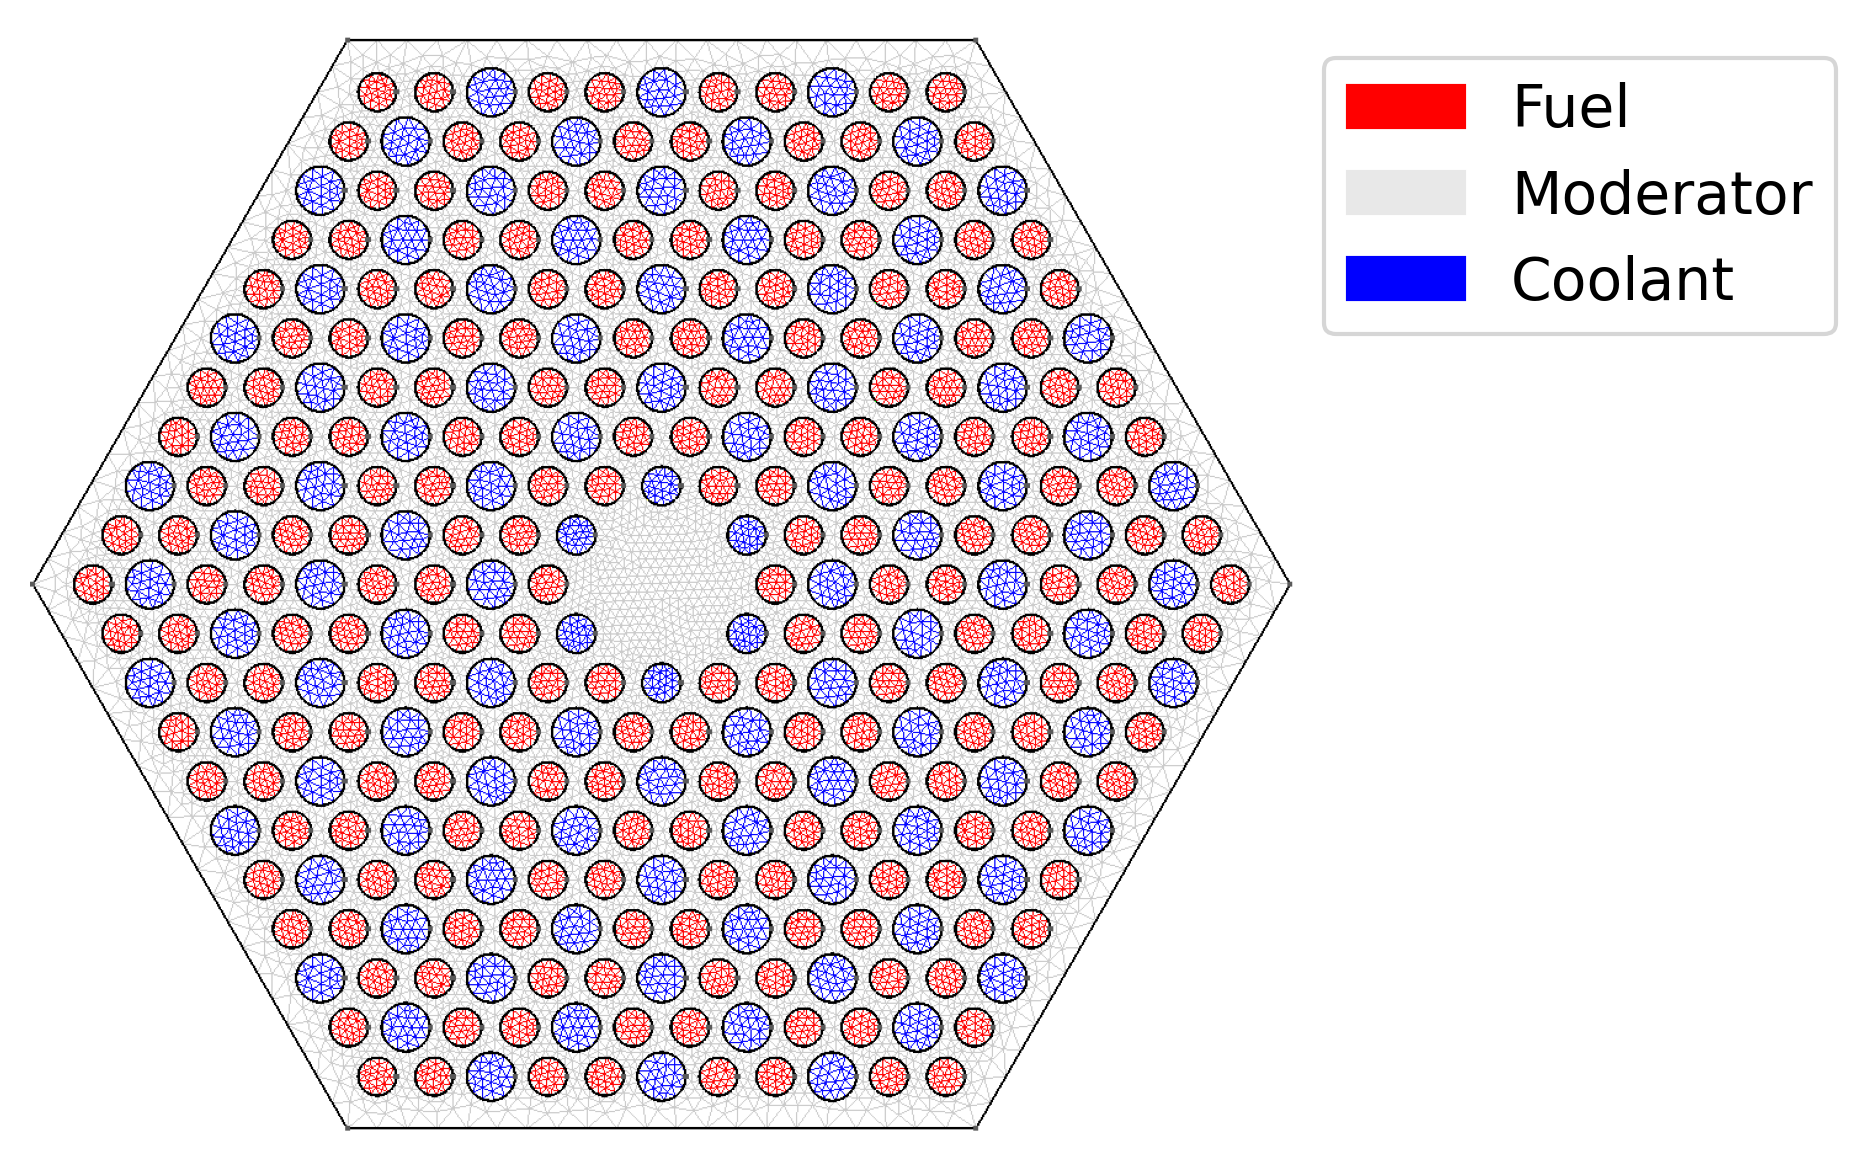
\includegraphics[width=0.45\linewidth]{figures-thermal/full-assem-mesh2}
  \hfill
  \caption{Full fuel column model geometry.}
  \label{fig:th-full-assem-mesh}
\end{figure}

% \begin{figure}[htbp!]
%   \centering
%     \subfloat[Model geometry.]{
%         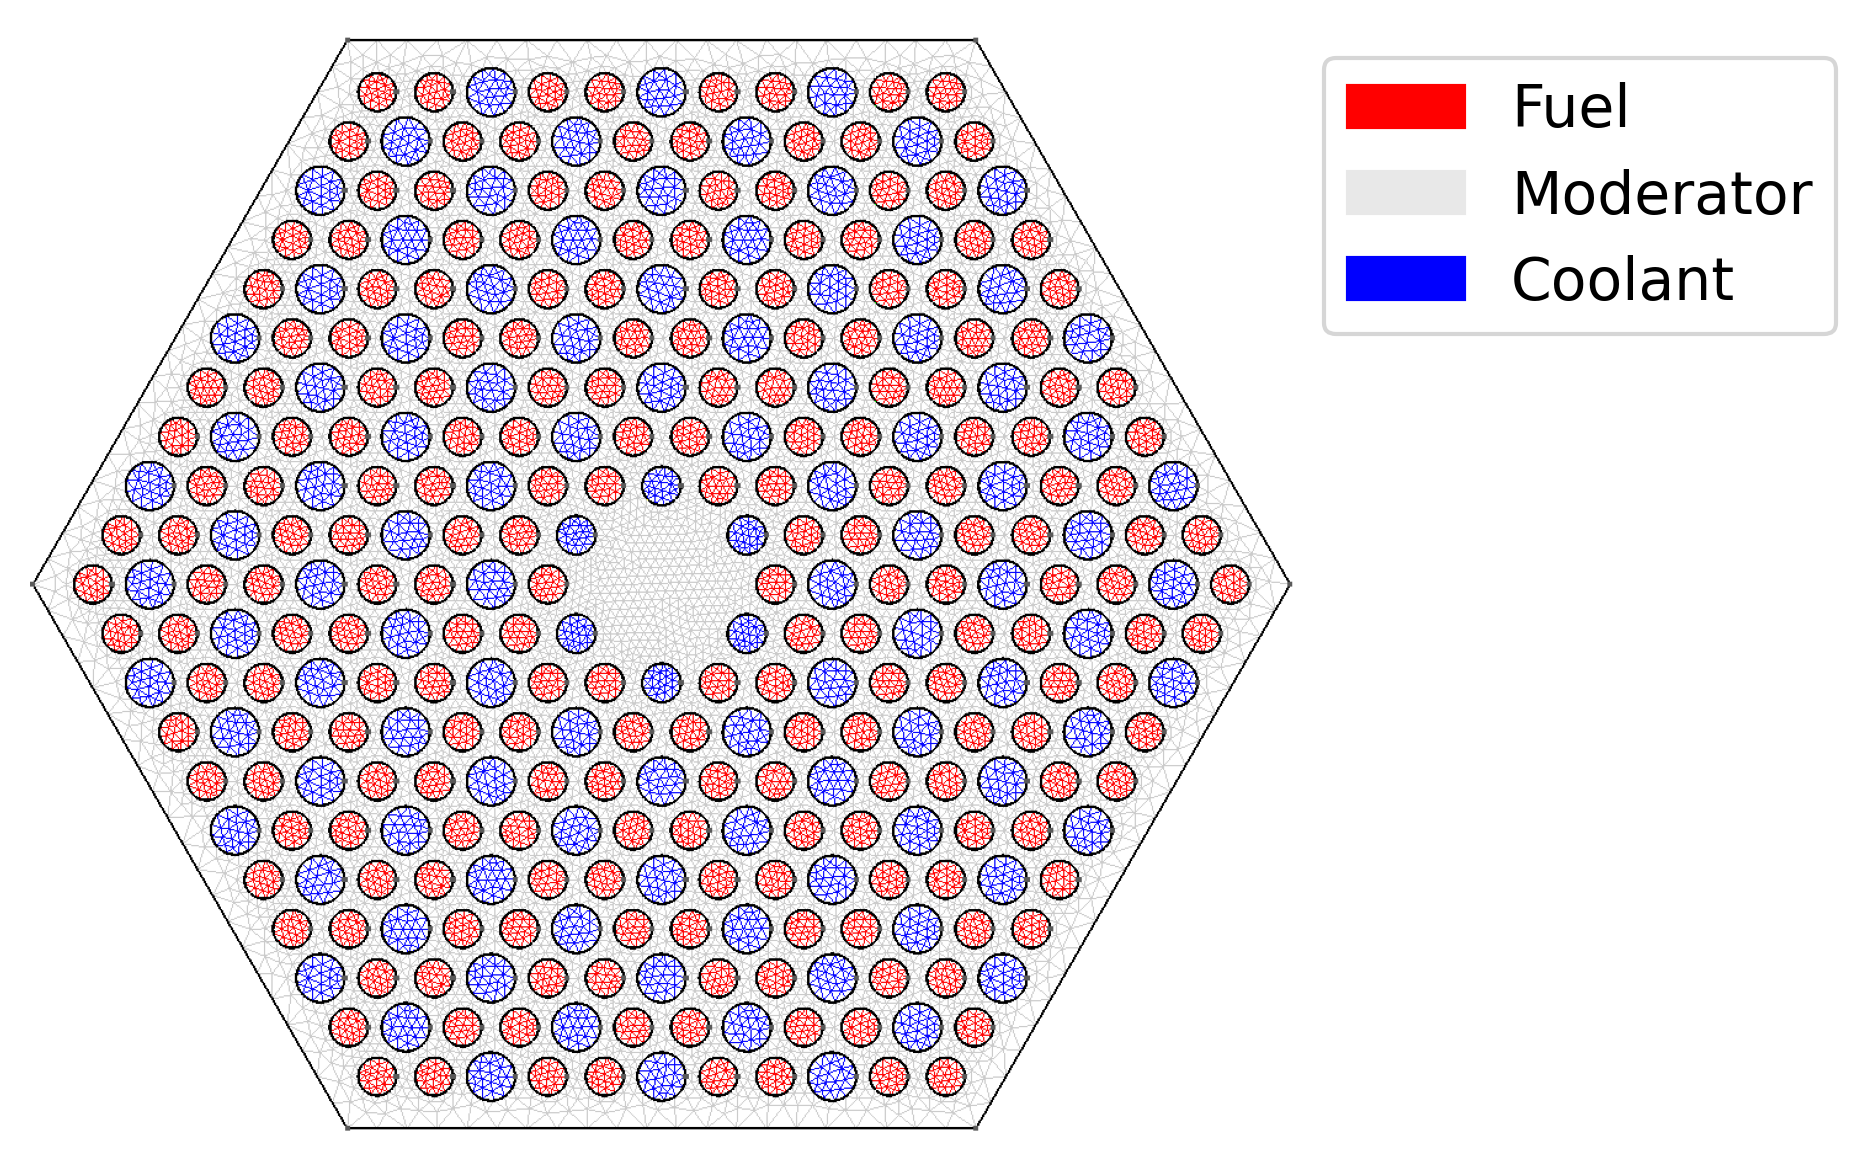
\includegraphics[width=0.45\textwidth]{figures-thermal/full-assem-mesh2}
%     }
%     \subfloat[Mesh convergence analysis.]{
%         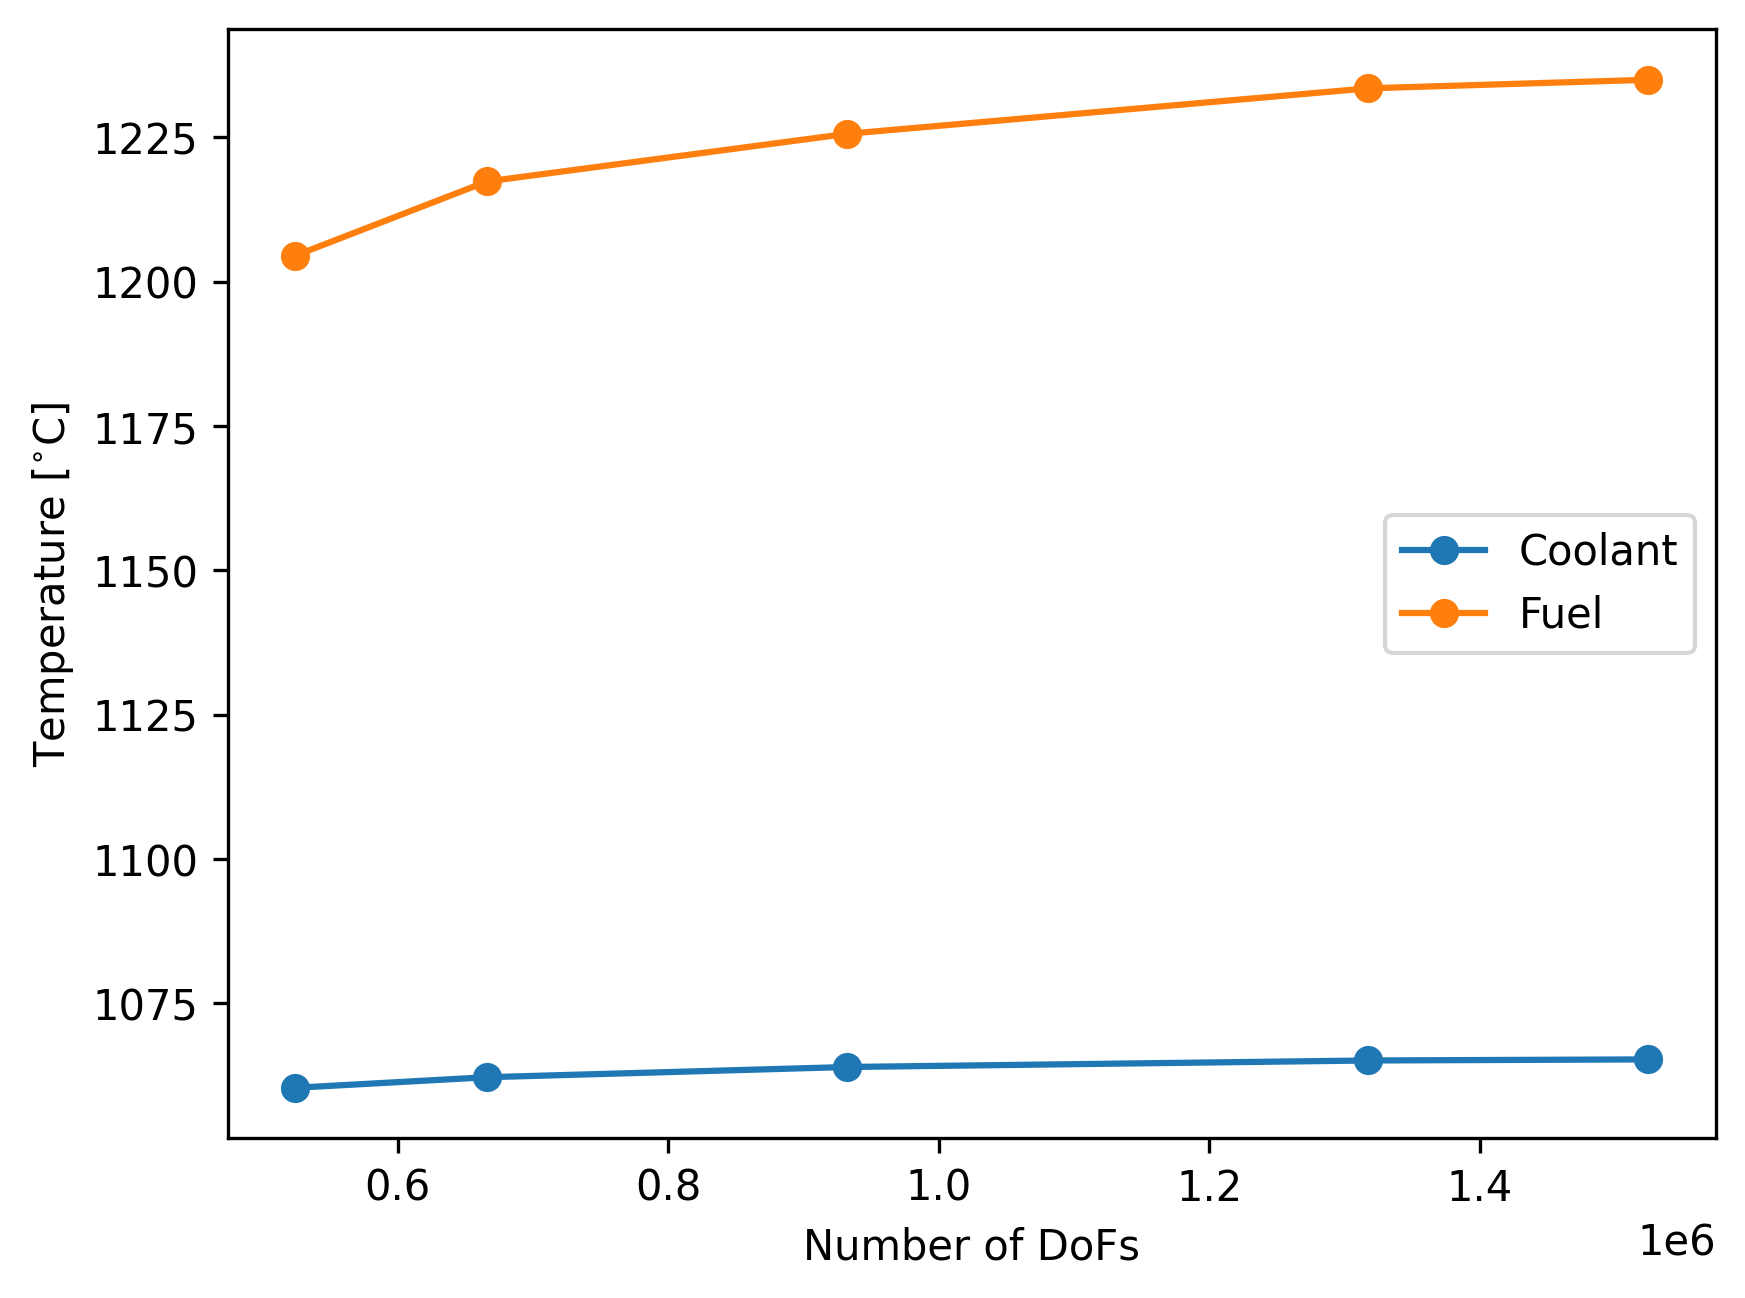
\includegraphics[width=0.45\textwidth]{figures-thermal/full-assem-convergence}
%     }
%   \hfill
%   \caption{Model geometry and mesh convergence analysis results.}
%   \label{fig:th-full-assem}
% \end{figure}

\begin{table}[htbp!]
  \centering
  \caption{Maximum temperatures.}
  \label{tab:th-full-assem-results}
\begin{tabular}{l|ccccc}
\toprule
                            & Mesh 1 & Mesh 2 & Mesh 3 & Mesh 4 & Mesh 5 \\
\midrule
Number of elements [$\times 10^{6}$]  & 1.025 & 1.306 & 1.833 & 2.596 & 3.006 \\
Number of DoFs [$\times 10^{6}$]      & 0.524 & 0.666 & 0.932 & 1.317 & 1.525 \\
Maximum coolant temperature & 1060.41 & 1062.23 & 1064.00 & 1065.13 & 1065.32 \\
Maximum fuel temperature    & 1204.49 & 1217.32 & 1225.57 & 1233.44 & 1234.93 \\
\bottomrule
\end{tabular}
\end{table}

% \section{Full-core 3D}
% This section will extend the methodology to a full-core problem and it will intend to solve Exercise 2 of Phase I of the OECD/NEA MHTGR-350 Benchmark.
% Trying \cite{stainsby_investigation_2008} approach.

\section{OECD/NEA MHTGR-350 MW Benchmark: Phase I Exercise 2}

This section conducted Phase I Exercise 2 of the benchamrk with Moltres/MOOSE.
OECD/NEA did not publish this exercise's results.
This section compares the results to INL's benchmark results \cite{strydom_inl_2013}.
Phase I Exercise 2 defines a thermal-fluids standalone calculation.
The benchmark specified the power density of each fuel region.
The exercise purpose is to ensure that the thermal-fluid model differences between participants are negligible and that they will not affect the coupled exercises.

Four sub-cases compose exercise 2:
\begin{itemize}
  \item Exercise 2a: No bypass flow and fixed thermophysical properties. No bypass flow modeled. The thermo-physical properties are constant.
  \item Exercise 2b: Bypass flow type I and fixed thermophysical properties. This exercise prescribes the bypass flow distribution. The thermo-physical properties are constant.
  \item Exercise 2c: Bypass flow type I and variable thermophysical properties. This exercise prescribes the bypass flow distribution. The thermo-physical properties depend on different simulation parameters.
  \item Exercise 2d: Bypass flow type II and variable thermophysical properties. This exercise solves the bypass flow distribution through the explicit modeling of the bypass gaps. The thermo-physical properties depend on different simulation parameters.
\end{itemize}

Modeling details/simplifications
* Mesh figure
* All the graphite regions assume the grade H-451 graphite material properties.


\begin{table}[htbp!]
\centering
      \caption{Material properties.}
      \label{tab:th-ex2a}
      \begin{tabular}{@{}l c S[table-format=2.2] c}
    \toprule
  \multicolumn{1}{c}{Parameter} & \multicolumn{1}{c@{}}{Value} & \multicolumn{1}{c@{}}{Units} & \multicolumn{1}{c}{Reference} \\    
    \midrule
  Fuel compact thermal conductivity & 20    & W/m/K   & \cite{oecd_nea_benchmark_2017} \\
  Fuel block thermal conductivity   & 37    & W/m/K   & \cite{oecd_nea_benchmark_2017} \\
  Graphite thermal conductivity     & 66    & W/m/K   & \cite{oecd_nea_benchmark_2017} \\
  \gls{RPV} thermal conductivity    & 40    & W/m/K   & \cite{oecd_nea_benchmark_2017} \\
  Coolant thermal conductivity      & 0.41  & W/m/K   & \cite{oecd_nea_benchmark_2017} \\
  Air thermal conductivity          & 0.068 & W/m/K   & \cite{oecd_nea_benchmark_2017} \\
  Helium density                    & $\times 10^{-6}$ & kg/cm$^3$ & \cite{nist_thermophysical_2020} \\
  Helium heat capacity              & 5188  & J/kg/K  & \cite{nist_thermophysical_2020} \\

    \midrule
  \multicolumn{1}{c}{Calculated parameters} &  &  &  & \\  
    \midrule
  Coolant film radius       & R$_i$ & 0.804    & cm     & -  \\
  Film thermal conductivity & k$_i$ & 2.09 $\times 10^{-3}$ & W/cm/K & -  \\
  \bottomrule
  \end{tabular}
\end{table}


Trying \cite{stainsby_investigation_2008} approach.

\section{Neutronics and Thermal-fluids Coupling}

Follow \cite{j_ortensi_initial_2012}.

3 options:
- Heterogeneous model
- Homogenized media and sub-channel unit cell model
- Porous media model

We chose:
- Heterogeneous model is computationally expensive

- Homogenized media and sub-channel unit cell model

'The initial coupling model was unable to correctly calculate the thermal coefficient in the fuel because it did not take into account the difference between the moderator and the fissile isotopes temperatures.
One of the major improvements of the coupling model is a de-homogenization calculation which guarantees a better description of the local thermal calculation in the fuel.' \cite{damian_vhtr_2008}.

Future work will analyze the possibility of using porous media in Moltres.
